\documentclass[10pt,ignorenonframetext,compress, aspectratio=169]{beamer}
\setbeamertemplate{caption}[numbered]
\setbeamertemplate{caption label separator}{: }
\setbeamercolor{caption name}{fg=normal text.fg}
\beamertemplatenavigationsymbolsempty
\usepackage{lmodern}
\usepackage{amssymb,amsmath,mathtools}
\usepackage{ifxetex,ifluatex}
\usepackage{fixltx2e} % provides \textsubscript
\ifnum 0\ifxetex 1\fi\ifluatex 1\fi=0 % if pdftex
  \usepackage[T1]{fontenc}
  \usepackage[utf8]{inputenc}
\else % if luatex or xelatex
  \ifxetex
    \usepackage{mathspec}
  \else
    \usepackage{fontspec}
  \fi
  %%\defaultfontfeatures{Ligatures=TeX,Scale=MatchLowercase}
  \defaultfontfeatures{Scale=MatchLowercase}
\fi
\usetheme[]{metropolis}
% use upquote if available, for straight quotes in verbatim environments
\IfFileExists{upquote.sty}{\usepackage{upquote}}{}
% use microtype if available
\IfFileExists{microtype.sty}{%
\usepackage{microtype}
\UseMicrotypeSet[protrusion]{basicmath} % disable protrusion for tt fonts
}{}
\newif\ifbibliography
\usepackage{color}
\usepackage{fancyvrb}
\newcommand{\VerbBar}{|}
\newcommand{\VERB}{\Verb[commandchars=\\\{\}]}
\DefineVerbatimEnvironment{Highlighting}{Verbatim}{commandchars=\\\{\}}
% Add ',fontsize=\small' for more characters per line
\usepackage{framed}
\definecolor{shadecolor}{RGB}{248,248,248}
\newenvironment{Shaded}{\begin{snugshade}}{\end{snugshade}}
\newcommand{\KeywordTok}[1]{\textcolor[rgb]{0.13,0.29,0.53}{\textbf{{#1}}}}
\newcommand{\DataTypeTok}[1]{\textcolor[rgb]{0.13,0.29,0.53}{{#1}}}
\newcommand{\DecValTok}[1]{\textcolor[rgb]{0.00,0.00,0.81}{{#1}}}
\newcommand{\BaseNTok}[1]{\textcolor[rgb]{0.00,0.00,0.81}{{#1}}}
\newcommand{\FloatTok}[1]{\textcolor[rgb]{0.00,0.00,0.81}{{#1}}}
\newcommand{\ConstantTok}[1]{\textcolor[rgb]{0.00,0.00,0.00}{{#1}}}
\newcommand{\CharTok}[1]{\textcolor[rgb]{0.31,0.60,0.02}{{#1}}}
\newcommand{\SpecialCharTok}[1]{\textcolor[rgb]{0.00,0.00,0.00}{{#1}}}
\newcommand{\StringTok}[1]{\textcolor[rgb]{0.31,0.60,0.02}{{#1}}}
\newcommand{\VerbatimStringTok}[1]{\textcolor[rgb]{0.31,0.60,0.02}{{#1}}}
\newcommand{\SpecialStringTok}[1]{\textcolor[rgb]{0.31,0.60,0.02}{{#1}}}
\newcommand{\ImportTok}[1]{{#1}}
\newcommand{\CommentTok}[1]{\textcolor[rgb]{0.56,0.35,0.01}{\textit{{#1}}}}
\newcommand{\DocumentationTok}[1]{\textcolor[rgb]{0.56,0.35,0.01}{\textbf{\textit{{#1}}}}}
\newcommand{\AnnotationTok}[1]{\textcolor[rgb]{0.56,0.35,0.01}{\textbf{\textit{{#1}}}}}
\newcommand{\CommentVarTok}[1]{\textcolor[rgb]{0.56,0.35,0.01}{\textbf{\textit{{#1}}}}}
\newcommand{\OtherTok}[1]{\textcolor[rgb]{0.56,0.35,0.01}{{#1}}}
\newcommand{\FunctionTok}[1]{\textcolor[rgb]{0.00,0.00,0.00}{{#1}}}
\newcommand{\VariableTok}[1]{\textcolor[rgb]{0.00,0.00,0.00}{{#1}}}
\newcommand{\ControlFlowTok}[1]{\textcolor[rgb]{0.13,0.29,0.53}{\textbf{{#1}}}}
\newcommand{\OperatorTok}[1]{\textcolor[rgb]{0.81,0.36,0.00}{\textbf{{#1}}}}
\newcommand{\BuiltInTok}[1]{{#1}}
\newcommand{\ExtensionTok}[1]{{#1}}
\newcommand{\PreprocessorTok}[1]{\textcolor[rgb]{0.56,0.35,0.01}{\textit{{#1}}}}
\newcommand{\AttributeTok}[1]{\textcolor[rgb]{0.77,0.63,0.00}{{#1}}}
\newcommand{\RegionMarkerTok}[1]{{#1}}
\newcommand{\InformationTok}[1]{\textcolor[rgb]{0.56,0.35,0.01}{\textbf{\textit{{#1}}}}}
\newcommand{\WarningTok}[1]{\textcolor[rgb]{0.56,0.35,0.01}{\textbf{\textit{{#1}}}}}
\newcommand{\AlertTok}[1]{\textcolor[rgb]{0.94,0.16,0.16}{{#1}}}
\newcommand{\ErrorTok}[1]{\textcolor[rgb]{0.64,0.00,0.00}{\textbf{{#1}}}}
\newcommand{\NormalTok}[1]{{#1}}

% Prevent slide breaks in the middle of a paragraph:
\widowpenalties 1 10000
\raggedbottom

\AtBeginPart{
  \let\insertpartnumber\relax
  \let\partname\relax
  \frame{\partpage}
}
\AtBeginSection{
  \ifbibliography
  \else
    \let\insertsectionnumber\relax
    \let\sectionname\relax
    \frame{\sectionpage}
  \fi
}
\AtBeginSubsection{
  \let\insertsubsectionnumber\relax
  \let\subsectionname\relax
  \frame{\subsectionpage}
}

\usepackage[normalem]{ulem}
% avoid problems with \sout in headers with hyperref:
\pdfstringdefDisableCommands{\renewcommand{\sout}{}}
\setlength{\parindent}{0pt}
\setlength{\parskip}{6pt plus 2pt minus 1pt}
\setlength{\emergencystretch}{3em}  % prevent overfull lines
\providecommand{\tightlist}{%
  \setlength{\itemsep}{0pt}\setlength{\parskip}{0pt}}
\setcounter{secnumdepth}{0}

%% GLS Added
% Textcomp for various common symbols
\usepackage{textcomp}

\usepackage{booktabs}

% Creative Commons Icons
\usepackage[scale=1]{ccicons}

\newenvironment{centrefig}{\begin{figure}\centering}{\end{figure}}
\newcommand{\columnsbegin}{\begin{columns}}
\newcommand{\columnsend}{\end{columns}}
\newcommand{\centreFigBegin}{\begin{figure}\centering}
\newcommand{\centreFigEnd}{\end{figure}}
%%

\DefineVerbatimEnvironment{Highlighting}{Verbatim}{commandchars=\\\{\}, fontsize=\tiny}
% make console-output smaller:
\makeatletter
\def\verbatim{\tiny\@verbatim \frenchspacing\@vobeyspaces \@xverbatim}
\makeatother
\setlength{\parskip}{0pt}
\setlength{\OuterFrameSep}{-4pt} % was -4pt
\makeatletter
\preto{\@verbatim}{\topsep=-10pt \partopsep=-10pt} % were -10pt
\makeatother

\title{Constrained Ordination}
\author{Gavin L. Simpson}
\date{U Adelaide 2017 • Feb 13--17 2017}

\begin{document}
\frame{\titlepage}

\section{Introduction}\label{introduction}

\begin{frame}{Introduction}

\end{frame}

\section{Constrained Ordination}\label{constrained-ordination}

\begin{frame}[fragile]{Canonical Correspondence Analysis}

CCA is the constrained form of CA; fitted using \texttt{cca()}.

Two interfaces for specifying models

\begin{itemize}
\tightlist
\item
  basic;
  \texttt{cca1\ \textless{}-\ cca(X\ =\ varespec,\ Y\ =\ varechem)}
\item
  formula;
  \texttt{cca1\ \textless{}-\ cca(varespec\ \textasciitilde{}\ .,\ data\ =\ varechem)}
\end{itemize}

Formula interface is the more powerful --- \emph{recommended}

\end{frame}

\begin{frame}[fragile]{Canonical Correspondence Analysis}

\tiny

\begin{Shaded}
\begin{Highlighting}[]
\NormalTok{cca1 <-}\StringTok{ }\KeywordTok{cca}\NormalTok{(varespec ~}\StringTok{ }\NormalTok{., }\DataTypeTok{data =} \NormalTok{varechem)}
\NormalTok{cca1}
\end{Highlighting}
\end{Shaded}

\begin{verbatim}
Call: cca(formula = varespec ~ N + P + K + Ca + Mg + S + Al + Fe +
Mn + Zn + Mo + Baresoil + Humdepth + pH, data = varechem)

              Inertia Proportion Rank
Total          2.0832     1.0000     
Constrained    1.4415     0.6920   14
Unconstrained  0.6417     0.3080    9
Inertia is mean squared contingency coefficient 

Eigenvalues for constrained axes:
  CCA1   CCA2   CCA3   CCA4   CCA5   CCA6   CCA7   CCA8   CCA9  CCA10 
0.4389 0.2918 0.1628 0.1421 0.1180 0.0890 0.0703 0.0584 0.0311 0.0133 
 CCA11  CCA12  CCA13  CCA14 
0.0084 0.0065 0.0062 0.0047 

Eigenvalues for unconstrained axes:
    CA1     CA2     CA3     CA4     CA5     CA6     CA7     CA8     CA9 
0.19776 0.14193 0.10117 0.07079 0.05330 0.03330 0.01887 0.01510 0.00949 
\end{verbatim}

\normalsize

\end{frame}

\begin{frame}[fragile]{Redundancy Analysis}

RDA is the constrained form of PCA; fitted using \texttt{rda()}.

\tiny

\begin{Shaded}
\begin{Highlighting}[]
\NormalTok{rda1 <-}\StringTok{ }\KeywordTok{rda}\NormalTok{(varespec ~}\StringTok{ }\NormalTok{., }\DataTypeTok{data =} \NormalTok{varechem)}
\NormalTok{rda1}
\end{Highlighting}
\end{Shaded}

\begin{verbatim}
Call: rda(formula = varespec ~ N + P + K + Ca + Mg + S + Al + Fe +
Mn + Zn + Mo + Baresoil + Humdepth + pH, data = varechem)

                Inertia Proportion Rank
Total         1825.6594     1.0000     
Constrained   1459.8891     0.7997   14
Unconstrained  365.7704     0.2003    9
Inertia is variance 

Eigenvalues for constrained axes:
 RDA1  RDA2  RDA3  RDA4  RDA5  RDA6  RDA7  RDA8  RDA9 RDA10 RDA11 RDA12 
820.1 399.3 102.6  47.6  26.8  24.0  19.1  10.2   4.4   2.3   1.5   0.9 
RDA13 RDA14 
  0.7   0.3 

Eigenvalues for unconstrained axes:
   PC1    PC2    PC3    PC4    PC5    PC6    PC7    PC8    PC9 
186.19  88.46  38.19  18.40  12.84  10.55   5.52   4.52   1.09 
\end{verbatim}

\normalsize

\end{frame}

\begin{frame}[fragile]{The \texttt{cca.object}}

\begin{itemize}
\tightlist
\item
  Objects of class \texttt{"cca"} are complex with many components
\item
  Entire class described in \texttt{?cca.object}
\item
  Depending on what analysis performed some components may be
  \texttt{NULL}
\item
  Used for (C)CA, PCA, RDA, and CAP (\texttt{capscale()})
\end{itemize}

\end{frame}

\begin{frame}[fragile]{The \texttt{cca.object}}

\texttt{cca1} has a large number of components

\begin{itemize}
\tightlist
\item
  \textbf{\texttt{\$call}} how the function was called
\item
  \textbf{\texttt{\$grand.total}} in (C)CA sum of `rowsum\}
\item
  \textbf{\texttt{\$rowsum}} the row sums
\item
  \textbf{\texttt{\$colsum}} the column sums
\item
  \textbf{\texttt{\$tot.chi}} total inertia, sum of Eigenvalues
\item
  \textbf{\texttt{\$pCCA}} Conditioned (partial-ed out) components
\item
  \textbf{\texttt{\$CCA}} Constrained components
\item
  \textbf{\texttt{\$CA}} Unconstrained components
\item
  \textbf{\texttt{\$method}} Ordination method used
\item
  \textbf{\texttt{\$inertia}} Description of what inertia is
\end{itemize}

\end{frame}

\begin{frame}[fragile]{The \texttt{cca.object}}

Depending on how one called \texttt{cca()} etc some of these components
will be \texttt{NULL}

\texttt{\$pCCA} is only filled in if a \emph{partial} constrained
ordination fitted

\texttt{rda()} returns objects with classes \texttt{"rda"} and
\texttt{"cca"}, but in most cases those objects work like those of class
\texttt{"cca"}

The Eigenvalues and axis scores are now spread about the \texttt{\$CA}
and \texttt{\$CCA} components (also \texttt{\$pCCA} if a \emph{partial}
CCA)

Thankfully we can use \emph{extractor} functions to get at such things

\end{frame}

\begin{frame}[fragile]{Eigenvalues}

Use \texttt{eigenvals()} to extract Eigenvalues from a fitted ordination
object

\scriptsize

\begin{Shaded}
\begin{Highlighting}[]
\KeywordTok{eigenvals}\NormalTok{(cca1)}
\end{Highlighting}
\end{Shaded}

\begin{verbatim}
     CCA1      CCA2      CCA3      CCA4      CCA5      CCA6      CCA7 
0.4388704 0.2917753 0.1628465 0.1421302 0.1179519 0.0890291 0.0702945 
     CCA8      CCA9     CCA10     CCA11     CCA12     CCA13     CCA14 
0.0583592 0.0311408 0.0132944 0.0083644 0.0065385 0.0061563 0.0047332 
      CA1       CA2       CA3       CA4       CA5       CA6       CA7 
0.1977645 0.1419256 0.1011741 0.0707868 0.0533034 0.0332994 0.0188676 
      CA8       CA9 
0.0151044 0.0094876 
\end{verbatim}

\normalsize

\end{frame}

\begin{frame}[fragile]{Your turn}

\begin{itemize}
\tightlist
\item
  Fit a CCA model to the lichen pasture data. The model should include,
  N, P, and K only.
\item
  Save the model in object \texttt{mycca1}
\item
  How much variance is explained by this model?
\item
  Extract the eigenvalues, how many constrained axes are there?
\end{itemize}

\begin{Shaded}
\begin{Highlighting}[]
\KeywordTok{library}\NormalTok{(}\StringTok{"vegan"}\NormalTok{)}
\KeywordTok{data}\NormalTok{(varechem, varespec)}
\NormalTok{## ...your code here...}
\end{Highlighting}
\end{Shaded}

\end{frame}

\begin{frame}[fragile]{Extracting axis scores}

To extract a range of scores from a fitted ordination use
\texttt{scores()}

\begin{itemize}
\tightlist
\item
  takes an ordination object as the first argument
\item
  \texttt{choices} --- which axes? Defaults to \texttt{c(1,2)}
\item
  \texttt{display} --- which type(s) of scores to return

  \begin{itemize}
  \tightlist
  \item
    \texttt{"sites"} or \texttt{"wa"}: scores for samples in response
    matrix
  \item
    \texttt{"species"}: scores for variables/columns in response
  \item
    \texttt{"lc"}: linear combination site scores
  \item
    \texttt{"bp"}: biplot scores (coords of arrow tip)
  \item
    \texttt{"cn"}: centroid scores (coords of factor centroids)
  \end{itemize}
\end{itemize}

\end{frame}

\begin{frame}[fragile]{Extracting axis scores}

\scriptsize

\begin{Shaded}
\begin{Highlighting}[]
\KeywordTok{str}\NormalTok{(}\KeywordTok{scores}\NormalTok{(cca1, }\DataTypeTok{choices =} \DecValTok{1}\NormalTok{:}\DecValTok{4}\NormalTok{, }\DataTypeTok{display =} \KeywordTok{c}\NormalTok{(}\StringTok{"species"}\NormalTok{,}\StringTok{"sites"}\NormalTok{)), }\DataTypeTok{max =} \DecValTok{1}\NormalTok{)}
\end{Highlighting}
\end{Shaded}

\begin{verbatim}
List of 2
 $ species: num [1:44, 1:4] 0.0753 -0.1813 -1.0535 -1.2774 -0.1526 ...
  ..- attr(*, "dimnames")=List of 2
 $ sites  : num [1:24, 1:4] 0.178 -0.97 -1.28 -1.501 -0.598 ...
  ..- attr(*, "dimnames")=List of 2
\end{verbatim}

\begin{Shaded}
\begin{Highlighting}[]
\KeywordTok{head}\NormalTok{(}\KeywordTok{scores}\NormalTok{(cca1, }\DataTypeTok{choices =} \DecValTok{1}\NormalTok{:}\DecValTok{2}\NormalTok{, }\DataTypeTok{display =} \StringTok{"sites"}\NormalTok{))}
\end{Highlighting}
\end{Shaded}

\begin{verbatim}
         CCA1       CCA2
18  0.1784733 -1.0598842
15 -0.9702382 -0.1971387
24 -1.2798478  0.4764498
27 -1.5009195  0.6521559
23 -0.5980933 -0.1840362
19 -0.1102881  0.7143142
\end{verbatim}

\normalsize

\end{frame}

\begin{frame}[fragile]{Scalings\ldots{}}

When we draw the results of many ordinations we display 2 or more sets
of data

Can't display all of these and maintain relationships between the scores

\emph{Solution} scale one set of scores relative to the other via the
\texttt{scaling} argument

\begin{itemize}
\tightlist
\item
  \texttt{scaling\ =\ 1} --- Focus on sites, scale site scores by
  \(\lambda_i\)
\item
  \texttt{scaling\ =\ 2} --- Focus on species, scale species scores by
  \(\lambda_i\)
\item
  \texttt{scaling\ =\ 3} --- Symmetric scaling, scale both scores by
  \(\sqrt{\lambda_i}\)
\item
  \texttt{scaling\ =\ -1} --- As above, but
\item
  \texttt{scaling\ =\ -2} --- For \texttt{cca()} multiply results by
  \(\sqrt{(1/(1-\lambda_i))}\)
\item
  \texttt{scaling\ =\ -3} --- this is Hill's scaling
\item
  \texttt{scaling\ \textless{}\ 0} --- For \texttt{rda()} divide species
  scores by species' \(\sigma\)
\item
  \texttt{scaling\ =\ 0} --- raw scores
\end{itemize}

\scriptsize

\begin{Shaded}
\begin{Highlighting}[]
\KeywordTok{scores}\NormalTok{(cca1, }\DataTypeTok{choices =} \DecValTok{1}\NormalTok{:}\DecValTok{2}\NormalTok{, }\DataTypeTok{display =} \StringTok{"species"}\NormalTok{, }\DataTypeTok{scaling =} \DecValTok{3}\NormalTok{)}
\end{Highlighting}
\end{Shaded}

\normalsize

\end{frame}

\begin{frame}[fragile]{Scalings\ldots{}}

Thankfully we can use alternative descrpitors to extract scores:

\begin{itemize}
\tightlist
\item
  \texttt{"none"}
\item
  \texttt{"sites"}
\item
  \texttt{"species"}
\item
  \texttt{"symmetric"}
\end{itemize}

Two modifiers select negative scores depending on whether the model is
CCA or RDA:

\begin{itemize}
\tightlist
\item
  \texttt{hill\ =\ TRUE}
\item
  \texttt{correlation\ =\ TRUE}
\end{itemize}

\end{frame}

\begin{frame}{Your turn}

\begin{itemize}
\tightlist
\item
  Using the CCA model you fitted, extract the site scores for axes 2 and
  3 with Hill's scaling
\end{itemize}

\end{frame}

\begin{frame}[fragile]{Partial constrained ordinations}

\emph{Partial} constrained ordinations remove the effect of one or more
variables \emph{then} fit model of interest

Argument \texttt{Z} is used for a data frame of variables to partial out

Or with the formula interface use the \texttt{Condition()} function

\scriptsize

\begin{Shaded}
\begin{Highlighting}[]
\NormalTok{pcca <-}\StringTok{ }\KeywordTok{cca}\NormalTok{(}\DataTypeTok{X =} \NormalTok{varespec,}
            \DataTypeTok{Y =} \NormalTok{varechem[, }\StringTok{"Ca"}\NormalTok{, }\DataTypeTok{drop =} \OtherTok{FALSE}\NormalTok{],}
            \DataTypeTok{Z =} \NormalTok{varechem[, }\StringTok{"pH"}\NormalTok{, }\DataTypeTok{drop =} \OtherTok{FALSE}\NormalTok{])}
\NormalTok{pcca <-}\StringTok{ }\KeywordTok{cca}\NormalTok{(varespec ~}\StringTok{ }\NormalTok{Ca +}\StringTok{ }\KeywordTok{Condition}\NormalTok{(pH), }\DataTypeTok{data =} \NormalTok{varechem) ## easier!}
\end{Highlighting}
\end{Shaded}

\normalsize

\end{frame}

\begin{frame}[fragile]{Triplots}

Triplots will generally produce a mess; we can really only display a
couple of bits approximately anyway Trying to cram three things in is a
recipe for a mess\ldots{} but we can do it

\scriptsize

\begin{Shaded}
\begin{Highlighting}[]
\KeywordTok{plot}\NormalTok{(cca1)}
\end{Highlighting}
\end{Shaded}

\begin{center}\includegraphics[width=0.5\linewidth]{02-constrained-ordination_files/figure-beamer/triplot-1-1} \end{center}

\normalsize

\end{frame}

\begin{frame}[fragile]{Your turn}

\begin{itemize}
\tightlist
\item
  Using \texttt{mycca}, draw a triplot of axes 2 and 3 with sites
  scaling
\item
  Use the help file \texttt{?plot.cca} to help you work out how to do
  this
\end{itemize}

\end{frame}

\begin{frame}[fragile]{Building constrained ordination models}

If we don't want to think it's easy to fit a poor model with many
constraints

That's what I did with \texttt{cca1} and \texttt{rda1}

Remember, CCA and RDA are \emph{just regression methods} --- everything
you know about regression applies here

A better approach is to \emph{think} about the important variables and
include only those

The formula interface allows you to create interaction or quadratic
terms easily (though be careful with latter)

It also handles factor or class constraints automatically unlike the
basic interface

\end{frame}

\begin{frame}[fragile]{Building constrained ordination models}

\scriptsize

\begin{Shaded}
\begin{Highlighting}[]
\NormalTok{vare.cca <-}\StringTok{ }\KeywordTok{cca}\NormalTok{(varespec ~}\StringTok{ }\NormalTok{Al +}\StringTok{ }\NormalTok{P*(K +}\StringTok{ }\NormalTok{Baresoil), }\DataTypeTok{data =} \NormalTok{varechem)}
\NormalTok{vare.cca}
\end{Highlighting}
\end{Shaded}

\begin{verbatim}
Call: cca(formula = varespec ~ Al + P * (K + Baresoil), data =
varechem)

              Inertia Proportion Rank
Total           2.083      1.000     
Constrained     1.046      0.502    6
Unconstrained   1.038      0.498   17
Inertia is mean squared contingency coefficient 

Eigenvalues for constrained axes:
  CCA1   CCA2   CCA3   CCA4   CCA5   CCA6 
0.3756 0.2342 0.1407 0.1323 0.1068 0.0561 

Eigenvalues for unconstrained axes:
    CA1     CA2     CA3     CA4     CA5     CA6     CA7     CA8 
0.27577 0.15411 0.13536 0.11803 0.08887 0.05511 0.04919 0.03781 
(Showed only 8 of all 17 unconstrained eigenvalues)
\end{verbatim}

\normalsize

\end{frame}

\begin{frame}[fragile]{Building constrained ordination models}

For CCA we have little choice but to do

\begin{enumerate}
\def\labelenumi{\arabic{enumi}.}
\tightlist
\item
  Fit well-chosen set of candidate models \& compare, or
\item
  Fit a \emph{full} model of well-chosen variables \& then do stepwise
  selection
\end{enumerate}

But automatic approaches to model building should be used cautiously!

The standard \texttt{step()} function can be used as \textbf{vegan}
provides two helper methods, \texttt{deviance()} and
\texttt{extractAIC()}, used by \texttt{step()}

Vegan also provides methods for class \texttt{"cca"} for \texttt{add1()}
and \texttt{drop1()}

\end{frame}

\begin{frame}[fragile]{Variance inflation factors}

\emph{Linear} dependencies between constraints can be investigated via
the \emph{variance inflation factor} or VIF

VIF is a measure of how much the variance of \(\hat{\beta}_j\) is
inflated by presence of other covariates

Lots of rules of thumb

\begin{itemize}
\tightlist
\item
  VIF \textgreater{}= 20 indicates \emph{strong collinearity} in
  constraints
\item
  VIF \textgreater{}= 10 potentially of concern \& should be looked at
\end{itemize}

Computed via \texttt{vif.cca()}

\end{frame}

\begin{frame}[fragile]{Stepwise selection in CCA}

\texttt{step()} uses AIC which is a fudge for RDA/CCA. Alternatively use
function \texttt{ordistep()}

\begin{enumerate}
\def\labelenumi{\arabic{enumi}.}
\tightlist
\item
  Define an upper and lower model scope, say the full model and the null
  model
\item
  To step from the lower scope or null model we use
\end{enumerate}

\scriptsize

\begin{Shaded}
\begin{Highlighting}[]
\NormalTok{upr <-}\StringTok{ }\KeywordTok{cca}\NormalTok{(varespec ~}\StringTok{ }\NormalTok{., }\DataTypeTok{data =} \NormalTok{varechem)}
\NormalTok{lwr <-}\StringTok{ }\KeywordTok{cca}\NormalTok{(varespec ~}\StringTok{ }\DecValTok{1}\NormalTok{, }\DataTypeTok{data =} \NormalTok{varechem)}
\KeywordTok{set.seed}\NormalTok{(}\DecValTok{1}\NormalTok{)}
\NormalTok{mods <-}\StringTok{ }\KeywordTok{ordistep}\NormalTok{(lwr, }\DataTypeTok{scope =} \KeywordTok{formula}\NormalTok{(upr), }\DataTypeTok{trace =} \DecValTok{0}\NormalTok{)}
\end{Highlighting}
\end{Shaded}

\normalsize

\texttt{trace\ =\ 0} is used her to turn off printing of progress

Permutation tests are used (more on these later); the theory for an AIC
for ordination is somewhat loose

\end{frame}

\begin{frame}[fragile]{Stepwise selection in CCA}

The object returned by \texttt{step()} is a standard \texttt{"cca"}
object with an extra component \texttt{\$anova}

The \texttt{\$anova} component contains a summary of the steps involved
in automatic model building

\tiny

\begin{Shaded}
\begin{Highlighting}[]
\NormalTok{mods}
\end{Highlighting}
\end{Shaded}

\begin{verbatim}
Call: cca(formula = varespec ~ Al + P + K, data = varechem)

              Inertia Proportion Rank
Total          2.0832     1.0000     
Constrained    0.6441     0.3092    3
Unconstrained  1.4391     0.6908   20
Inertia is mean squared contingency coefficient 

Eigenvalues for constrained axes:
  CCA1   CCA2   CCA3 
0.3616 0.1700 0.1126 

Eigenvalues for unconstrained axes:
   CA1    CA2    CA3    CA4    CA5    CA6    CA7    CA8 
0.3500 0.2201 0.1851 0.1551 0.1351 0.1003 0.0773 0.0537 
(Showed only 8 of all 20 unconstrained eigenvalues)
\end{verbatim}

\normalsize

\end{frame}

\begin{frame}[fragile]{Stepwise selection in CCA}

The \texttt{\$anova} component contains a summary of the steps involved
in automatic model building

\scriptsize

\begin{Shaded}
\begin{Highlighting}[]
\NormalTok{mods$anova}
\end{Highlighting}
\end{Shaded}

\begin{verbatim}
     Df    AIC      F Pr(>F)   
+ Al  1 128.61 3.6749  0.005 **
+ P   1 127.91 2.5001  0.005 **
+ K   1 127.44 2.1688  0.035 * 
---
Signif. codes:  0 '***' 0.001 '**' 0.01 '*' 0.05 '.' 0.1 ' ' 1
\end{verbatim}

\normalsize

\end{frame}

\begin{frame}[fragile]{Stepwise selection in CCA}

Step-wise model selection is fairly fragile; if we start from the full
model we won't end up with the same final model

\tiny

\begin{Shaded}
\begin{Highlighting}[]
\NormalTok{mods2 <-}\StringTok{ }\KeywordTok{step}\NormalTok{(upr, }\DataTypeTok{scope =} \KeywordTok{list}\NormalTok{(}\DataTypeTok{lower =} \KeywordTok{formula}\NormalTok{(lwr), }\DataTypeTok{upper =} \KeywordTok{formula}\NormalTok{(upr)), }\DataTypeTok{trace =} \DecValTok{0}\NormalTok{,}
              \DataTypeTok{test =} \StringTok{"perm"}\NormalTok{)}
\NormalTok{mods2}
\end{Highlighting}
\end{Shaded}

\begin{verbatim}
Call: cca(formula = varespec ~ P + K + Mg + S + Mn + Mo + Baresoil
+ Humdepth, data = varechem)

              Inertia Proportion Rank
Total          2.0832     1.0000     
Constrained    1.1165     0.5360    8
Unconstrained  0.9667     0.4640   15
Inertia is mean squared contingency coefficient 

Eigenvalues for constrained axes:
  CCA1   CCA2   CCA3   CCA4   CCA5   CCA6   CCA7   CCA8 
0.4007 0.2488 0.1488 0.1266 0.0875 0.0661 0.0250 0.0130 

Eigenvalues for unconstrained axes:
    CA1     CA2     CA3     CA4     CA5     CA6     CA7     CA8     CA9 
0.25821 0.18813 0.11927 0.10204 0.08791 0.06085 0.04461 0.02782 0.02691 
   CA10    CA11    CA12    CA13    CA14    CA15 
0.01646 0.01364 0.00823 0.00655 0.00365 0.00238 
\end{verbatim}

\normalsize

\end{frame}

\begin{frame}[fragile]{Adjusted \(R^2\) for \emph{linear} models}

As with ordinary \(R^2\), that of an RDA is biased for the same reasons
as for a linear regression

\begin{itemize}
\tightlist
\item
  adding a variable to constraints will increase \(R^2\)
\item
  the larger the number of constraints in the model the larger \(R^2\)
  is due to random correlations
\end{itemize}

Can attempt to account for this bias via an \emph{adjusted} \(R^2\)
measure

\[R^2_{adj} = 1 - \frac{n - 1}{n - m - 1}(1 - R^2)\]

\begin{itemize}
\tightlist
\item
  \(n\) is number of samples \(m\) is number of constraints (model
  degrees of freedom)
\item
  Can be used up to \(\sim M > n/2\) before becomes too conservative
\item
  Can be negative
\item
  Compute using \texttt{RsquareAdj()}
\end{itemize}

\end{frame}

\begin{frame}[fragile]{Stepwise selection via adjusted \(R^2\)}

The problems with stepwise selection in regression models are myriad.
Affects RDA, CCA, etc as well

Blanchet, Legendre, and Borcard (2008) proposed a two-step solution for
models where \(R^2_{adj}\) makes sense

\begin{itemize}
\tightlist
\item
  \emph{Global test} of all constraints

  \begin{itemize}
  \tightlist
  \item
    Proceed \textbf{only} if this test is significant
  \item
    Helps prevent inflation of overall type I error
  \end{itemize}
\item
  Proceed with forward selection, but with \emph{two} stopping rules

  \begin{itemize}
  \tightlist
  \item
    Usual significance threshold \(\alpha\)
  \item
    The global \(R^2_{adj}\)
  \item
    Stop if next candidate model is non-significant or if \(R^2_{adj}\)
    exceeds the global \(R^2_{adj}\)
  \end{itemize}
\end{itemize}

Available in \texttt{ordiR2step()}

\end{frame}

\section{Permutation tests}\label{permutation-tests}

\begin{frame}{Permutation tests in vegan}

RDA has lots of theory behind it, CCA not as much. However,
ecological/environmental data invariably violate what little theory we
have

Instead we use permutation tests to assess the \emph{importance} of
fitted models --- the data are shuffled in some way and the model
refitted to derive a Null distribution under some hypothesis of \emph{no
effect}

\end{frame}

\begin{frame}[fragile]{Permutation tests in vegan}

What \emph{is} shuffled and \emph{how} is of \textbf{paramount}
importance for the test to be valid

\begin{itemize}
\tightlist
\item
  No conditioning (partial) variables then rows of the species data are
  permuted
\item
  With conditioning variables, two options are available, both of which
  \emph{permute residuals} from model fits

  \begin{itemize}
  \tightlist
  \item
    The \emph{full model} uses residuals from model
    \(Y = X + Z + \varepsilon\)
  \item
    The \emph{reduced model} uses residuals from model
    \(Y = X + Z + \varepsilon\)
  \end{itemize}
\item
  In \textbf{vegan} which is used can be set via argument \texttt{model}
  with \texttt{"direct"}, \sout{\texttt{"full"}}, and \texttt{"reduced"}
  respectively
\item
  In current \textbf{vegan} option \texttt{method\ =\ "full"} is
  disabled
\end{itemize}

\end{frame}

\begin{frame}{Permutation tests in vegan}

A test statistic is required, computed for observed model \& each
permuted model

\textbf{vegan} uses a pseudo-\(F\) statistic

\[F=\frac{\chi^2_{model} / df_{model}}{\chi^2_{resid} / df_{resid}}\]

Evaluate whether \(F\) is unusually large relative to the null
(permutation) distribution of \(F\)

\end{frame}

\begin{frame}[fragile]{Permutation tests in vegan: \texttt{anova()}}

\begin{itemize}
\tightlist
\item
  The main user function is the \texttt{anova()} method
\item
  It is an interface to the lower-level function
  \texttt{permutest.cca()}
\item
  At its most simplest, the \texttt{anova()} method tests whether the
  ``model'' as a whole is significant
  \[F = \frac{1.4415 / 14}{0.6417 / 9} = 1.4441\]
\end{itemize}

\tiny

\begin{Shaded}
\begin{Highlighting}[]
\KeywordTok{set.seed}\NormalTok{(}\DecValTok{42}\NormalTok{)}
\NormalTok{(perm <-}\StringTok{ }\KeywordTok{anova}\NormalTok{(cca1))}
\end{Highlighting}
\end{Shaded}

\begin{verbatim}
Permutation test for cca under reduced model
Permutation: free
Number of permutations: 999

Model: cca(formula = varespec ~ N + P + K + Ca + Mg + S + Al + Fe + Mn + Zn + Mo + Baresoil + Humdepth + pH, data = varechem)
         Df ChiSquare      F Pr(>F)  
Model    14   1.44148 1.4441  0.041 *
Residual  9   0.64171                
---
Signif. codes:  0 '***' 0.001 '**' 0.01 '*' 0.05 '.' 0.1 ' ' 1
\end{verbatim}

\normalsize

\end{frame}

\begin{frame}[fragile]{Permutation tests in vegan: \texttt{anova()}}

\begin{itemize}
\tightlist
\item
  \texttt{anova.cca()} has a number of arguments
\end{itemize}

\tiny

\begin{Shaded}
\begin{Highlighting}[]
\KeywordTok{args}\NormalTok{(anova.cca)}
\end{Highlighting}
\end{Shaded}

\begin{verbatim}
function (object, ..., permutations = how(nperm = 999), by = NULL, 
    model = c("reduced", "direct", "full"), parallel = getOption("mc.cores"), 
    strata = NULL, cutoff = 1, scope = NULL) 
NULL
\end{verbatim}

\normalsize

\begin{itemize}
\tightlist
\item
  \texttt{object} is the fitted ordination
\item
  \texttt{permutations} controls what is permuted and how
\item
  \texttt{by} determines what is tested; the default is to test the
  model
\end{itemize}

\end{frame}

\begin{frame}[fragile]{Types of permutation test in vegan}

A number of types of test can be envisaged

\begin{itemize}
\tightlist
\item
  Testing the overall significance of the model
\item
  Testing constrained (canonical) axes
\item
  Testing individual model terms \emph{sequentially}
\item
  The \emph{marginal} effect of a single variable
\end{itemize}

The first is the default in \texttt{anova()}

The other three can be selected via the argument \texttt{by}

\end{frame}

\begin{frame}[fragile]{Permutation tests \textbar{} testing canonical
axes}

\begin{itemize}
\tightlist
\item
  The constrained (canonical) axes can be individually tests by
  specifying \texttt{by\ =\ "axis"}
\item
  The first axis is tested in terms of variance explained compared to
  residual variance
\item
  The second axis is tested after partialling out the first axis\ldots{}
  and so on
\end{itemize}

\tiny

\begin{Shaded}
\begin{Highlighting}[]
\KeywordTok{set.seed}\NormalTok{(}\DecValTok{1}\NormalTok{)}
\KeywordTok{anova}\NormalTok{(mods, }\DataTypeTok{by =} \StringTok{"axis"}\NormalTok{)}
\end{Highlighting}
\end{Shaded}

\begin{verbatim}
Permutation test for cca under reduced model
Marginal tests for axes
Permutation: free
Number of permutations: 999

Model: cca(formula = varespec ~ Al + P + K, data = varechem)
         Df ChiSquare      F Pr(>F)    
CCA1      1   0.36156 5.0249  0.001 ***
CCA2      1   0.16996 2.3621  0.011 *  
CCA3      1   0.11262 1.5651  0.124    
Residual 20   1.43906                  
---
Signif. codes:  0 '***' 0.001 '**' 0.01 '*' 0.05 '.' 0.1 ' ' 1
\end{verbatim}

\normalsize

\end{frame}

\begin{frame}[fragile]{Permutation tests \textbar{} testing terms
sequentially}

\begin{itemize}
\tightlist
\item
  The individual terms in the model can be tested using
  \texttt{by\ =\ "terms"}
\item
  The terms are assessed in the order they were specified in the model,
  sequentially from first to last
\item
  Test is of the additional variance explained by adding the \(k\)th
  variable to the model
\item
  \textbf{Ordering of the terms} will affect the results
\end{itemize}

\tiny

\begin{Shaded}
\begin{Highlighting}[]
\KeywordTok{set.seed}\NormalTok{(}\DecValTok{5}\NormalTok{)}
\KeywordTok{anova}\NormalTok{(mods, }\DataTypeTok{by =} \StringTok{"terms"}\NormalTok{)}
\end{Highlighting}
\end{Shaded}

\begin{verbatim}
Permutation test for cca under reduced model
Terms added sequentially (first to last)
Permutation: free
Number of permutations: 999

Model: cca(formula = varespec ~ Al + P + K, data = varechem)
         Df ChiSquare      F Pr(>F)    
Al        1   0.29817 4.1440  0.001 ***
P         1   0.18991 2.6393  0.011 *  
K         1   0.15605 2.1688  0.024 *  
Residual 20   1.43906                  
---
Signif. codes:  0 '***' 0.001 '**' 0.01 '*' 0.05 '.' 0.1 ' ' 1
\end{verbatim}

\normalsize

\end{frame}

\begin{frame}[fragile]{Permutation tests \textbar{} testing terms
marginal effects}

\begin{itemize}
\tightlist
\item
  The marginal \emph{effect} of a model term can be assessed using
  \texttt{by\ =\ "margin"}
\item
  The marginal \emph{effect} is the effect of a particular term when all
  other model terms are included in the model
\end{itemize}

\tiny

\begin{Shaded}
\begin{Highlighting}[]
\KeywordTok{set.seed}\NormalTok{(}\DecValTok{10}\NormalTok{)}
\KeywordTok{anova}\NormalTok{(mods, }\DataTypeTok{by =} \StringTok{"margin"}\NormalTok{)}
\end{Highlighting}
\end{Shaded}

\begin{verbatim}
Permutation test for cca under reduced model
Marginal effects of terms
Permutation: free
Number of permutations: 999

Model: cca(formula = varespec ~ Al + P + K, data = varechem)
         Df ChiSquare      F Pr(>F)    
Al        1   0.31184 4.3340  0.001 ***
P         1   0.16810 2.3362  0.012 *  
K         1   0.15605 2.1688  0.025 *  
Residual 20   1.43906                  
---
Signif. codes:  0 '***' 0.001 '**' 0.01 '*' 0.05 '.' 0.1 ' ' 1
\end{verbatim}

\normalsize

\end{frame}

\section{Your turn - Spring meadows}\label{your-turn---spring-meadows}

\begin{frame}[fragile]{Constrained ordination worked example \textbar{}
spring meadow vegetation}

Example \& data taken from Leps \& Smilauer, Case Study 2

Spring fen meadow vegetation in westernmost Carpathian mountains

\scriptsize

\begin{Shaded}
\begin{Highlighting}[]
\NormalTok{## load vegan}
\KeywordTok{library}\NormalTok{(}\StringTok{"vegan"}\NormalTok{)}

\NormalTok{## load the data}
\NormalTok{spp <-}\StringTok{ }\KeywordTok{read.csv}\NormalTok{(}\StringTok{"../00-data-sets/meadow-spp.csv"}\NormalTok{, }\DataTypeTok{header =} \OtherTok{TRUE}\NormalTok{, }\DataTypeTok{row.names =} \DecValTok{1}\NormalTok{)}
\NormalTok{env <-}\StringTok{ }\KeywordTok{read.csv}\NormalTok{(}\StringTok{"../00-data-sets/meadow-env.csv"}\NormalTok{, }\DataTypeTok{header =} \OtherTok{TRUE}\NormalTok{, }\DataTypeTok{row.names =} \DecValTok{1}\NormalTok{)}
\end{Highlighting}
\end{Shaded}

\normalsize

\end{frame}

\begin{frame}[fragile]{Constrained ordination worked example \textbar{}
spring meadow vegetation}

CCA a reasonable starting point as the gradient is long here (check with
\texttt{decorana()} if you want)

\scriptsize

\begin{Shaded}
\begin{Highlighting}[]
\NormalTok{m1 <-}\StringTok{ }\KeywordTok{cca}\NormalTok{(spp ~}\StringTok{ }\NormalTok{., }\DataTypeTok{data =} \NormalTok{env)}
\KeywordTok{set.seed}\NormalTok{(}\DecValTok{32}\NormalTok{)}
\KeywordTok{anova}\NormalTok{(m1)}
\end{Highlighting}
\end{Shaded}

\begin{verbatim}
Permutation test for cca under reduced model
Permutation: free
Number of permutations: 999

Model: cca(formula = spp ~ Ca + Mg + Fe + K + Na + Si + SO4 + PO4 + NO3 + NH3 + Cl + Corg + pH + conduct + slope, data = env)
         Df ChiSquare     F Pr(>F)    
Model    15    1.5597 1.497  0.001 ***
Residual 54    3.7509                 
---
Signif. codes:  0 '***' 0.001 '**' 0.01 '*' 0.05 '.' 0.1 ' ' 1
\end{verbatim}

\normalsize

\end{frame}

\begin{frame}[fragile]{Constrained ordination worked example \textbar{}
spring meadow vegetation}

\scriptsize

\begin{Shaded}
\begin{Highlighting}[]
\KeywordTok{plot}\NormalTok{(m1)}
\end{Highlighting}
\end{Shaded}

\begin{center}\includegraphics[width=0.5\linewidth]{02-constrained-ordination_files/figure-beamer/meadows-cca-full-triplot-1} \end{center}

\normalsize

\end{frame}

\begin{frame}[fragile]{Constrained ordination worked example \textbar{}
spring meadow vegetation}

\tiny

\begin{Shaded}
\begin{Highlighting}[]
\KeywordTok{set.seed}\NormalTok{(}\DecValTok{67}\NormalTok{)}
\NormalTok{lwr <-}\StringTok{ }\KeywordTok{cca}\NormalTok{(spp ~}\StringTok{ }\DecValTok{1}\NormalTok{, }\DataTypeTok{data =} \NormalTok{env)}
\NormalTok{m2 <-}\StringTok{ }\KeywordTok{ordistep}\NormalTok{(lwr, }\DataTypeTok{scope =} \KeywordTok{formula}\NormalTok{(m1), }\DataTypeTok{trace =} \OtherTok{FALSE}\NormalTok{)}
\end{Highlighting}
\end{Shaded}

\begin{Shaded}
\begin{Highlighting}[]
\NormalTok{m2}
\end{Highlighting}
\end{Shaded}

\begin{verbatim}
Call: cca(formula = spp ~ Ca + conduct + Corg + Na + NH3 + Fe +
pH, data = env)

              Inertia Proportion Rank
Total          5.3107     1.0000     
Constrained    0.9899     0.1864    7
Unconstrained  4.3208     0.8136   62
Inertia is mean squared contingency coefficient 

Eigenvalues for constrained axes:
  CCA1   CCA2   CCA3   CCA4   CCA5   CCA6   CCA7 
0.4268 0.1447 0.1116 0.0936 0.0760 0.0719 0.0652 

Eigenvalues for unconstrained axes:
    CA1     CA2     CA3     CA4     CA5     CA6     CA7     CA8 
0.27251 0.19518 0.16703 0.14993 0.14606 0.14168 0.13292 0.12154 
(Showed only 8 of all 62 unconstrained eigenvalues)
\end{verbatim}

\normalsize

\end{frame}

\begin{frame}[fragile]{Constrained ordination worked example \textbar{}
spring meadow vegetation}

\scriptsize

\begin{Shaded}
\begin{Highlighting}[]
\KeywordTok{plot}\NormalTok{(m2)}
\end{Highlighting}
\end{Shaded}

\begin{center}\includegraphics[width=0.5\linewidth]{02-constrained-ordination_files/figure-beamer/meadows-cca-reduced-triplot-1} \end{center}

\normalsize

\end{frame}

\begin{frame}[fragile]{Constrained ordination worked example \textbar{}
spring meadow vegetation}

\scriptsize

\begin{Shaded}
\begin{Highlighting}[]
\NormalTok{m2$anova}
\end{Highlighting}
\end{Shaded}

\begin{verbatim}
          Df    AIC      F Pr(>F)   
+ Ca       1 453.14 4.7893  0.005 **
+ conduct  1 453.29 1.7915  0.005 **
+ Corg     1 453.61 1.6011  0.005 **
+ Na       1 453.93 1.5827  0.005 **
+ NH3      1 454.36 1.4507  0.020 * 
+ Fe       1 454.89 1.3386  0.015 * 
+ pH       1 455.46 1.2756  0.015 * 
---
Signif. codes:  0 '***' 0.001 '**' 0.01 '*' 0.05 '.' 0.1 ' ' 1
\end{verbatim}

\normalsize

\end{frame}

\begin{frame}[fragile]{Constrained ordination worked example \textbar{}
spring meadow vegetation}

Alternative is RDA with a transformation

\scriptsize

\begin{Shaded}
\begin{Highlighting}[]
\NormalTok{spph <-}\StringTok{ }\KeywordTok{decostand}\NormalTok{(spp, }\DataTypeTok{method =} \StringTok{"hellinger"}\NormalTok{)}
\NormalTok{m3 <-}\StringTok{ }\KeywordTok{rda}\NormalTok{(spph ~}\StringTok{ }\NormalTok{., }\DataTypeTok{data =} \NormalTok{env)}
\NormalTok{lwr <-}\StringTok{ }\KeywordTok{rda}\NormalTok{(spph ~}\StringTok{ }\DecValTok{1}\NormalTok{, }\DataTypeTok{data =} \NormalTok{env)}
\NormalTok{m4 <-}\StringTok{ }\KeywordTok{ordistep}\NormalTok{(lwr, }\DataTypeTok{scope =} \KeywordTok{formula}\NormalTok{(m3), }\DataTypeTok{trace =} \OtherTok{FALSE}\NormalTok{)}
\end{Highlighting}
\end{Shaded}

\normalsize

\end{frame}

\begin{frame}[fragile]{Constrained ordination worked example \textbar{}
spring meadow vegetation}

\scriptsize

\begin{Shaded}
\begin{Highlighting}[]
\KeywordTok{plot}\NormalTok{(m4)}
\end{Highlighting}
\end{Shaded}

\begin{center}\includegraphics[width=0.5\linewidth]{02-constrained-ordination_files/figure-beamer/meadows-rda-reduced-triplot-1} \end{center}

\normalsize

\end{frame}

\begin{frame}[fragile]{Constrained ordination worked example \textbar{}
spring meadow vegetation}

Stepwise using \(R^2_{adj}\)

\scriptsize

\begin{Shaded}
\begin{Highlighting}[]
\NormalTok{m5 <-}\StringTok{ }\KeywordTok{ordiR2step}\NormalTok{(lwr, }\DataTypeTok{scope =} \KeywordTok{formula}\NormalTok{(m3), }\DataTypeTok{trace =} \OtherTok{FALSE}\NormalTok{)}
\NormalTok{m5$anova}
\end{Highlighting}
\end{Shaded}

\begin{verbatim}
                 R2.adj Df     AIC       F Pr(>F)   
+ Ca            0.12588  1 -41.779 10.9370  0.002 **
+ NH3           0.14628  1 -42.468  2.6242  0.002 **
+ conduct       0.16322  1 -42.925  2.3570  0.002 **
+ Si            0.17711  1 -43.164  2.1136  0.002 **
+ Corg          0.18518  1 -42.940  1.6442  0.006 **
+ NO3           0.19257  1 -42.680  1.5853  0.018 * 
+ pH            0.19966  1 -42.417  1.5583  0.010 **
<All variables> 0.20332                             
---
Signif. codes:  0 '***' 0.001 '**' 0.01 '*' 0.05 '.' 0.1 ' ' 1
\end{verbatim}

\normalsize

\end{frame}

\section{Restricted permutation
tests}\label{restricted-permutation-tests}

\begin{frame}{Restricted permutation tests}

What \emph{is} shuffled and \emph{how} is of \textbf{paramount}
importance for the test to be valid

Complete randomisation (default in \textbf{vegan}) assumes a null
hypothesis where all observations are \emph{independent}

Ecological / environmental data often aren't independent

\begin{itemize}
\tightlist
\item
  Temporal or spatial correlation
\item
  Clustering, repeated measures
\item
  Nested sampling designs (Split-plots designs)
\item
  Blocks
\item
  \ldots{}
\end{itemize}

Permutation \emph{must} give null distribution of the test statistic
whilst preserving the \emph{dependence} between observations

Trick is to shuffle the data whilst preserving that dependence

\end{frame}

\begin{frame}[fragile]{Restricted permutations}

Canoco has had restricted permutations for a \emph{long} time.
\textbf{vegan} has only recently caught up \& we're not (quite) there
yet

\textbf{vegan} used to only know how to completely randomise data or
completely randomise within blocks (via \texttt{strata} in
\textbf{vegan})

The newish package \textbf{permute} grew out of initial code in the
\textbf{vegan} repository to generate the sorts of restricted
permutations available in Canoco

We have now fully integrated \textbf{permute} into
\textbf{vegan}\ldots{}

\textbf{vegan} depends on \textbf{permute} so it will already be
installed \& loaded when using \textbf{vegan}

\end{frame}

\begin{frame}{Restricted permutations with permute}

\textbf{permute} follows Canoco closely --- at the chiding of Cajo ter
Braak when it didn't do what he wanted!

Samples can be thought of as belonging to three levels of a hierarchy

\begin{itemize}
\tightlist
\item
  the \emph{sample} level; how are individual samples permuted
\item
  the \emph{plot} level; how are samples grouped at an intermediate
  level
\item
  the \emph{block} level; how are samples grouped at the outermost level
\end{itemize}

Blocks define groups of plots, each of which can contain groups of
samples

\end{frame}

\begin{frame}{Restricted permutations with permute}

Blocks are \emph{never} permuted; if defined, only plots or samples
\emph{within} the blocks get shuffled \& samples are \textbf{never}
swapped between blocks

Plots or samples within plots, or both can be permuted following one of
four simple permutation types

\begin{enumerate}
\def\labelenumi{\arabic{enumi}.}
\tightlist
\item
  Free permutation (randomisation)
\item
  Time series or linear transect, equal spacing
\item
  Spatial grid designs, equal regular spacing
\item
  Permutation of plots (groups of samples)
\item
  Fixed (no permutation)
\end{enumerate}

Multiple plots per block, multiple samples per plot; plots could be
arranged in a spatial grid and samples within each of the plots form a
time series

\end{frame}

\begin{frame}[fragile]{Restricted permutations with permute \textbar{}
blocks}

Blocks are a random factor that does not interact with factors that vary
within blocks

Blocks form groups of samples that are never permuted between blocks,
only within blocks

Using blocks you can achieve what the \texttt{strata} argument used to
in \textbf{vegan}; needs to be a factor variable

The variation \emph{between} blocks should be excluded from the test;
\textbf{permute} doesn't do this for you!

Use \texttt{+\ Condition(blocks)} in the model formula where
\texttt{blocks} is a factor containing the block membership for each
observation

\end{frame}

\begin{frame}{Restricted permutations with permute \textbar{} time
series \& linear transects}

Can link \emph{randomly} starting point of one series to any time point
of another series if series are stationary under null hypothesis that
the series are unrelated

Achieve this via cyclic shift permutations --- wrap series into a circle
by joining start and end points

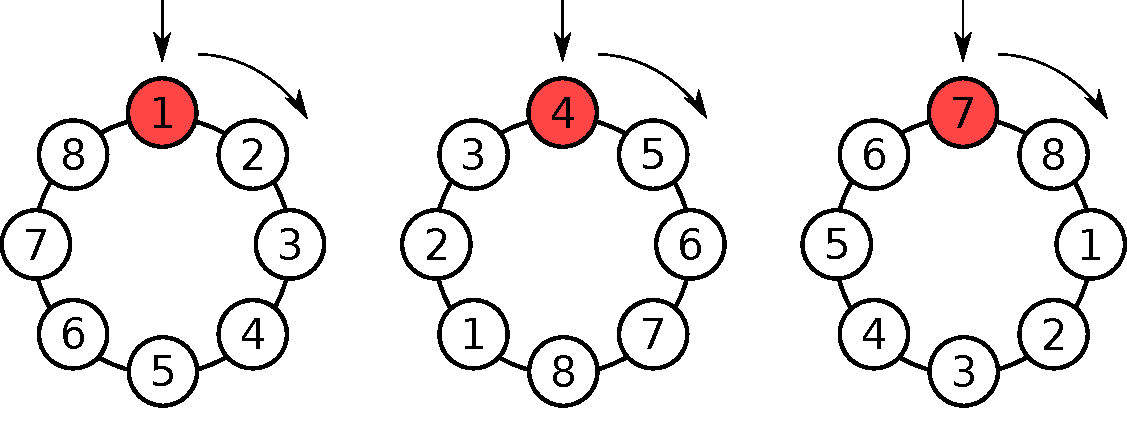
\includegraphics[width=\linewidth]{cyclic-shifts-figure}

\end{frame}

\begin{frame}[fragile]{Restricted permutations with permute \textbar{}
time series \& linear transects}

Works OK if there are no trends or cyclic pattern --- autocorrelation
structure only broken at the end points \emph{if} series are stationary

Can detrend to make series stationary but not if you want to test
significance of a trend

\scriptsize

\begin{Shaded}
\begin{Highlighting}[]
\KeywordTok{shuffle}\NormalTok{(}\DecValTok{10}\NormalTok{, }\DataTypeTok{control =} \KeywordTok{how}\NormalTok{(}\DataTypeTok{within =} \KeywordTok{Within}\NormalTok{(}\DataTypeTok{type =} \StringTok{"series"}\NormalTok{)))}
\end{Highlighting}
\end{Shaded}

\begin{verbatim}
 [1]  9 10  1  2  3  4  5  6  7  8
\end{verbatim}

\normalsize

\end{frame}

\begin{frame}[fragile]{Restricted permutations with permute \textbar{}
spatial grids}

\columnsbegin
\column{0.5\linewidth} The trick of cyclic shifts can be extended to two
dimensions for a regular spatial grid arrangement of points

Now shifts are \emph{toroidal} as we join the end point in the \emph{x}
direction together and in the \emph{y} direction together

\scriptsize

\begin{Shaded}
\begin{Highlighting}[]
\KeywordTok{matrix}\NormalTok{(perm, }\DataTypeTok{ncol =} \DecValTok{3}\NormalTok{)}
\end{Highlighting}
\end{Shaded}

\begin{verbatim}
     [,1] [,2] [,3]
[1,]    6    9    3
[2,]    4    7    1
[3,]    5    8    2
\end{verbatim}

\normalsize

\column{0.5\linewidth}
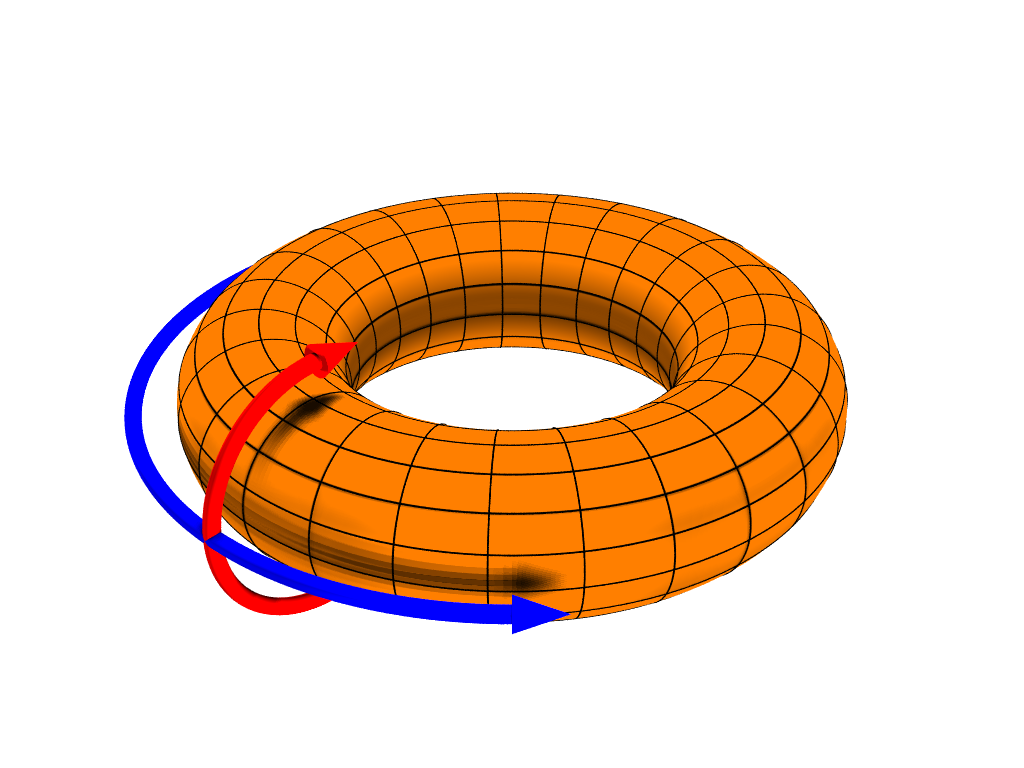
\includegraphics[width=\linewidth]{Toroidal_coord}

Source: Dave Burke, Wikimedia \ccby
\columnsend

\end{frame}

\begin{frame}{Restricted permutations with permute \textbar{}
whole-plots \& split-plots I}

Split-plot designs are hierarchical with two levels of units

\begin{enumerate}
\def\labelenumi{\arabic{enumi}.}
\tightlist
\item
  \textbf{whole-plots} , which contain
\item
  \textbf{split-plots} (the samples)
\end{enumerate}

Can permute one or both of these but whole-plots must be of equal size

Essentially allows more than one error stratum to be analyzed

Test effect of constraints that vary \emph{between} whole plots by
permuting the whole-plots whilst retaining order of split-splots
(samples) within the whole-plots

Test effect of constraints that vary \emph{within} whole-plots by
permuting the split-plots within whole-plots without permuting the
whole-plots

\end{frame}

\begin{frame}[fragile]{Restricted permutations with permute \textbar{}
whole-plots \& split-plots II}

Whole-plots or split-plots can be time series, linear transects or
rectangular grids in which case the appropriate restricted permutation
is used

If the split-plots are parallel time series \& \texttt{time} is an
autocorrelated error component affecting all series then the same cyclic
shift can be applied to each time series (within each whole-plot)
(\texttt{constant\ =\ TRUE})

\end{frame}

\begin{frame}{Restricted permutations with permute \textbar{} mirroring}

Mirroring in restricted permutations allows for isotropy in dependencies
by reflecting the ordering of samples in time or spatial dimensions

For a linear transect, technically the autocorrelation at lag \emph{h}
is equal to that at lag -\emph{h} (also in a trend-free time series)

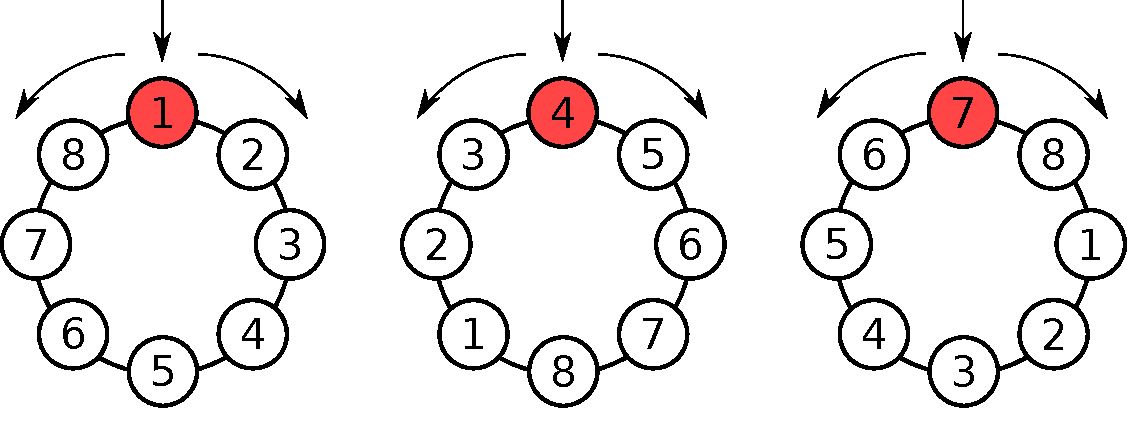
\includegraphics[width=\linewidth]{cyclic-shifts-with-mirror-figure}

\end{frame}

\begin{frame}[fragile]{Restricted permutations with permute \textbar{}
mirroring}

Hence the series \texttt{(1,\ 2,\ 3,\ 4)} and \texttt{(4,\ 3,\ 2,\ 1)}
are equivalent fom this point of view \& we can draw permutations from
either version

Similar argument can be made for spatial grids

Using \texttt{mirror\ =\ TRUE} then can double (time series, linear
transects) or quadruple (spatial grids) the size of the set of
permutations

\end{frame}

\begin{frame}[fragile]{Restricted permutations with permute \textbar{}
the set of permutations}

Using restricted permutations can severely reduce the size of the set of
allowed permutations

As the minimum \emph{p} value obtainable is \(1 / np\) where \(np\) is
number of allowed permutations (including the observed) this can impact
the ability to detect signal/pattern

If we don't want mirroring

\begin{itemize}
\tightlist
\item
  in a time series of 20 samples the minimum \emph{p} is 1/20 (0.05)
\item
  in a time series of 100 samples the minimum \emph{p} is 1/100 (0.01)
\item
  in a data set with 10 time series each of 20 observations (200 total),
  if we assume an autocorrelated error component over all series
  (\texttt{constant\ =\ TRUE}) then there are only 20 permutations of
  the data and minimum \emph{p} is 0.05
\end{itemize}

When the set of permutations is small it is better to switch to an exact
test \& evaluate all permutations in the set rather than randomly sample
from the set

\end{frame}

\begin{frame}[fragile]{Restricted permutations with permute \textbar{}
designing permutation schemes}

In \textbf{permute}, we set up a permutation scheme with \texttt{how()}

We sample from the permutation scheme with

\begin{itemize}
\tightlist
\item
  \texttt{shuffle()}, which gives a single draw from scheme, or
\item
  \texttt{shuffleSet()}, which returns a set of \texttt{n} draws from
  the scheme
\end{itemize}

\texttt{allPerms()} can generated the entire set of permutations ---
\textbf{note} this was designed for small sets of permutations \& is
slow if you request it for a scheme with many thousands of permutations!

\end{frame}

\begin{frame}[fragile]{Restricted permutations with permute \textbar{}
designing permutation schemes}

\texttt{how()} has three main arguments

\begin{enumerate}
\def\labelenumi{\arabic{enumi}.}
\tightlist
\item
  \texttt{within} --- takes input from helper \texttt{Within()}
\item
  \texttt{plots} --- takes input from helper \texttt{Plots()}
\item
  \texttt{blocks} --- takes a factor variable as input
\end{enumerate}

\scriptsize

\begin{Shaded}
\begin{Highlighting}[]
\NormalTok{plt <-}\StringTok{ }\KeywordTok{gl}\NormalTok{(}\DecValTok{3}\NormalTok{, }\DecValTok{10}\NormalTok{)}
\NormalTok{h <-}\StringTok{ }\KeywordTok{how}\NormalTok{(}\DataTypeTok{within =} \KeywordTok{Within}\NormalTok{(}\DataTypeTok{type =} \StringTok{"series"}\NormalTok{), }\DataTypeTok{plots =} \KeywordTok{Plots}\NormalTok{(}\DataTypeTok{strata =} \NormalTok{plt))}
\end{Highlighting}
\end{Shaded}

\normalsize

\end{frame}

\begin{frame}[fragile]{Restricted permutations with permute \textbar{}
designing permutation schemes}

Helper functions make it easy to change one or a few aspects of
permutation scheme, rest left at defaults

\scriptsize

\begin{Shaded}
\begin{Highlighting}[]
\KeywordTok{args}\NormalTok{(Within)}
\end{Highlighting}
\end{Shaded}

\begin{verbatim}
function (type = c("free", "series", "grid", "none"), constant = FALSE, 
    mirror = FALSE, ncol = NULL, nrow = NULL) 
NULL
\end{verbatim}

\begin{Shaded}
\begin{Highlighting}[]
\KeywordTok{args}\NormalTok{(Plots)}
\end{Highlighting}
\end{Shaded}

\begin{verbatim}
function (strata = NULL, type = c("none", "free", "series", "grid"), 
    mirror = FALSE, ncol = NULL, nrow = NULL) 
NULL
\end{verbatim}

\normalsize

\end{frame}

\begin{frame}[fragile]{Restricted permutations with permute \textbar{}
designing permutation schemes}

\texttt{how()} has additional arguments, many of which control the
heuristics that kick in to stop you shooting yourself in the foot and
demanding 9999 permutations when there are only 10

\begin{itemize}
\tightlist
\item
  \texttt{complete} should we enumerate the entire set of permutations?
\item
  \texttt{minperm} lower bound on the size of the set of permutations at
  \& below which we turn on complete enumeration
\end{itemize}

\scriptsize

\begin{Shaded}
\begin{Highlighting}[]
\KeywordTok{args}\NormalTok{(how)}
\end{Highlighting}
\end{Shaded}

\begin{verbatim}
function (within = Within(), plots = Plots(), blocks = NULL, 
    nperm = 199, complete = FALSE, maxperm = 9999, minperm = 5040, 
    all.perms = NULL, make = TRUE, observed = FALSE) 
NULL
\end{verbatim}

\normalsize

\end{frame}

\begin{frame}[fragile]{Restricted permutations with permute \textbar{}
time series example I}

Time series within 3 plots, 10 observation each

\scriptsize

\begin{Shaded}
\begin{Highlighting}[]
\NormalTok{plt <-}\StringTok{ }\KeywordTok{gl}\NormalTok{(}\DecValTok{3}\NormalTok{, }\DecValTok{10}\NormalTok{)}
\NormalTok{h <-}\StringTok{ }\KeywordTok{how}\NormalTok{(}\DataTypeTok{within =} \KeywordTok{Within}\NormalTok{(}\DataTypeTok{type =} \StringTok{"series"}\NormalTok{),}
         \DataTypeTok{plots =} \KeywordTok{Plots}\NormalTok{(}\DataTypeTok{strata =} \NormalTok{plt))}
\KeywordTok{set.seed}\NormalTok{(}\DecValTok{4}\NormalTok{)}
\NormalTok{p <-}\StringTok{ }\KeywordTok{shuffle}\NormalTok{(}\DecValTok{30}\NormalTok{, }\DataTypeTok{control =} \NormalTok{h)}
\KeywordTok{do.call}\NormalTok{(}\StringTok{"rbind"}\NormalTok{, }\KeywordTok{split}\NormalTok{(p, plt)) ## look at perms in context}
\end{Highlighting}
\end{Shaded}

\begin{verbatim}
  [,1] [,2] [,3] [,4] [,5] [,6] [,7] [,8] [,9] [,10]
1    7    8    9   10    1    2    3    4    5     6
2   12   13   14   15   16   17   18   19   20    11
3   24   25   26   27   28   29   30   21   22    23
\end{verbatim}

\normalsize

\end{frame}

\begin{frame}[fragile]{Restricted permutations with permute \textbar{}
time series example II}

Time series within 3 plots, 10 observation each, same permutation within
each

\scriptsize

\begin{Shaded}
\begin{Highlighting}[]
\NormalTok{plt <-}\StringTok{ }\KeywordTok{gl}\NormalTok{(}\DecValTok{3}\NormalTok{, }\DecValTok{10}\NormalTok{)}
\NormalTok{h <-}\StringTok{ }\KeywordTok{how}\NormalTok{(}\DataTypeTok{within =} \KeywordTok{Within}\NormalTok{(}\DataTypeTok{type =} \StringTok{"series"}\NormalTok{, }\DataTypeTok{constant =} \OtherTok{TRUE}\NormalTok{),}
         \DataTypeTok{plots =} \KeywordTok{Plots}\NormalTok{(}\DataTypeTok{strata =} \NormalTok{plt))}
\KeywordTok{set.seed}\NormalTok{(}\DecValTok{4}\NormalTok{)}
\NormalTok{p <-}\StringTok{ }\KeywordTok{shuffle}\NormalTok{(}\DecValTok{30}\NormalTok{, }\DataTypeTok{control =} \NormalTok{h)}
\KeywordTok{do.call}\NormalTok{(}\StringTok{"rbind"}\NormalTok{, }\KeywordTok{split}\NormalTok{(p, plt)) ## look at perms in context}
\end{Highlighting}
\end{Shaded}

\begin{verbatim}
  [,1] [,2] [,3] [,4] [,5] [,6] [,7] [,8] [,9] [,10]
1    7    8    9   10    1    2    3    4    5     6
2   17   18   19   20   11   12   13   14   15    16
3   27   28   29   30   21   22   23   24   25    26
\end{verbatim}

\normalsize

\end{frame}

\section{Ohraz Case Study}\label{ohraz-case-study}

\begin{frame}[fragile]{Restricted permutations with permute \textbar{}
worked example with vegan}

Now we've seen how to drive \textbf{permute}, we can use the same
\texttt{how()} commands to set up permutation designs within
\textbf{vegan} functions

Analyse the Ohraz data Case study 5 of Leps \& Smilauer

Repeated observations of composition from an experiment

\begin{itemize}
\tightlist
\item
  Factorial design (3 replicates)
\item
  Treatments: fertilisation, mowing, \emph{Molinia} removal
\end{itemize}

Test 1 of the hypotheses

\begin{quote}
There are \emph{no} directional changes in species composition in time
that are common to all treatments or specific treatments
\end{quote}

\end{frame}

\begin{frame}[fragile]{Restricted permutations with permute \textbar{}
worked example with vegan}

Analyse the Ohraz data Case study 5 of Leps \& Smilauer

\scriptsize

\begin{Shaded}
\begin{Highlighting}[]
\NormalTok{## load vegan}
\KeywordTok{library}\NormalTok{(}\StringTok{"vegan"}\NormalTok{)}

\NormalTok{## load the data}
\NormalTok{spp <-}\StringTok{ }\KeywordTok{read.csv}\NormalTok{(}\StringTok{"../00-data-sets/ohraz-spp.csv"}\NormalTok{, }\DataTypeTok{header =} \OtherTok{TRUE}\NormalTok{, }\DataTypeTok{row.names =} \DecValTok{1}\NormalTok{)}
\NormalTok{env <-}\StringTok{ }\KeywordTok{read.csv}\NormalTok{(}\StringTok{"../00-data-sets/ohraz-env.csv"}\NormalTok{, }\DataTypeTok{header =} \OtherTok{TRUE}\NormalTok{, }\DataTypeTok{row.names =} \DecValTok{1}\NormalTok{)}
\NormalTok{molinia <-}\StringTok{ }\NormalTok{spp[, }\DecValTok{1}\NormalTok{]}
\NormalTok{spp <-}\StringTok{ }\NormalTok{spp[, -}\DecValTok{1}\NormalTok{]}

\NormalTok{## Year as numeric}
\NormalTok{env <-}\StringTok{ }\KeywordTok{transform}\NormalTok{(env, }\DataTypeTok{year =} \KeywordTok{as.numeric}\NormalTok{(}\KeywordTok{as.character}\NormalTok{(year)))}
\end{Highlighting}
\end{Shaded}

\normalsize

\end{frame}

\begin{frame}[fragile]{Restricted permutations with permute \textbar{}
worked example with vegan}

\scriptsize

\begin{Shaded}
\begin{Highlighting}[]
\NormalTok{c1 <-}\StringTok{ }\KeywordTok{rda}\NormalTok{(spp ~}\StringTok{ }\NormalTok{year +}\StringTok{ }\NormalTok{year:mowing +}\StringTok{ }\NormalTok{year:fertilizer +}\StringTok{ }\NormalTok{year:removal +}\StringTok{ }\KeywordTok{Condition}\NormalTok{(plotid), }\DataTypeTok{data =} \NormalTok{env)}
\NormalTok{(h <-}\StringTok{ }\KeywordTok{how}\NormalTok{(}\DataTypeTok{within =} \KeywordTok{Within}\NormalTok{(}\DataTypeTok{type =} \StringTok{"none"}\NormalTok{), }\DataTypeTok{plots =} \KeywordTok{Plots}\NormalTok{(}\DataTypeTok{strata =} \NormalTok{env$plotid, }\DataTypeTok{type =} \StringTok{"free"}\NormalTok{)))}
\end{Highlighting}
\end{Shaded}

\begin{verbatim}

Permutation Design:

Blocks:
  Defined by: none

Plots:
  Plots: env$plotid
  Permutation type: free
  Mirrored?: No

Within Plots:
  Permutation type: none

Permutation details:
  Number of permutations: 199
  Max. number of permutations allowed: 9999
  Evaluate all permutations?: No.  Activation limit: 5040
\end{verbatim}

\end{frame}

\begin{frame}[fragile]{Restricted permutations with permute \textbar{}
worked example with vegan}

\scriptsize

\begin{Shaded}
\begin{Highlighting}[]
\KeywordTok{set.seed}\NormalTok{(}\DecValTok{42}\NormalTok{)}
\KeywordTok{anova}\NormalTok{(c1, }\DataTypeTok{permutations =} \NormalTok{h, }\DataTypeTok{model =} \StringTok{"reduced"}\NormalTok{)}
\end{Highlighting}
\end{Shaded}

\begin{verbatim}
Permutation test for rda under reduced model
Plots: env$plotid, plot permutation: free
Permutation: none
Number of permutations: 199

Model: rda(formula = spp ~ year + year:mowing + year:fertilizer + year:removal + Condition(plotid), data = env)
         Df Variance      F Pr(>F)   
Model     4   158.85 6.4247  0.005 **
Residual 90   556.30                 
---
Signif. codes:  0 '***' 0.001 '**' 0.01 '*' 0.05 '.' 0.1 ' ' 1
\end{verbatim}

\end{frame}

\begin{frame}[fragile]{Restricted permutations with permute \textbar{}
worked example with vegan}

\scriptsize

\begin{Shaded}
\begin{Highlighting}[]
\KeywordTok{set.seed}\NormalTok{(}\DecValTok{24}\NormalTok{)}
\KeywordTok{anova}\NormalTok{(c1, }\DataTypeTok{permutations =} \NormalTok{h, }\DataTypeTok{model =} \StringTok{"reduced"}\NormalTok{, }\DataTypeTok{by =} \StringTok{"axis"}\NormalTok{)}
\end{Highlighting}
\end{Shaded}

\begin{verbatim}
Permutation test for rda under reduced model
Marginal tests for axes
Plots: env$plotid, plot permutation: free
Permutation: none
Number of permutations: 199

Model: rda(formula = spp ~ year + year:mowing + year:fertilizer + year:removal + Condition(plotid), data = env)
         Df Variance       F Pr(>F)   
RDA1      1    89.12 14.4173  0.005 **
RDA2      1    34.28  5.5458  0.005 **
RDA3      1    26.52  4.2900  0.010 **
RDA4      1     8.94  1.4458  0.650   
Residual 90   556.30                  
---
Signif. codes:  0 '***' 0.001 '**' 0.01 '*' 0.05 '.' 0.1 ' ' 1
\end{verbatim}

\normalsize

\end{frame}

\section{Hierarchical analysis of
crayfish}\label{hierarchical-analysis-of-crayfish}

\begin{frame}{Hierarchical analysis of crayfish}

Variation in communities may exist at various scales, sometimes
hierarchically

A firt step in understanding this variation is to test for its
exisistence

In this example from Leps \& Smilauer (2014) uses crayfish data from
Spring River, Arkansas/Missouri, USA, collected by
Dr.\textasciitilde{}Camille Flinders.

567 records of 5 species (each sub-divided into \emph{Large} \&
\emph{Small} individuals

\end{frame}

\begin{frame}[fragile]{Hierarchical analysis of crayfish}

\begin{Shaded}
\begin{Highlighting}[]
\NormalTok{## load data}
\NormalTok{crayfish <-}\StringTok{ }\KeywordTok{head}\NormalTok{(}\KeywordTok{read.csv}\NormalTok{(}\StringTok{"../00-data-sets/crayfish-spp.csv"}\NormalTok{)[, -}\DecValTok{1}\NormalTok{], -}\DecValTok{1}\NormalTok{)}
\NormalTok{design <-}\StringTok{ }\KeywordTok{read.csv}\NormalTok{(}\StringTok{"../00-data-sets/crayfish-design.csv"}\NormalTok{, }\DataTypeTok{skip =} \DecValTok{1}\NormalTok{)[, -}\DecValTok{1}\NormalTok{]}

\NormalTok{## fixup the names}
\KeywordTok{names}\NormalTok{(crayfish) <-}\StringTok{ }\KeywordTok{gsub}\NormalTok{(}\StringTok{"}\CharTok{\textbackslash{}\textbackslash{}}\StringTok{."}\NormalTok{, }\StringTok{""}\NormalTok{, }\KeywordTok{names}\NormalTok{(crayfish))}
\KeywordTok{names}\NormalTok{(design) <-}\StringTok{ }\KeywordTok{c}\NormalTok{(}\StringTok{"Watershed"}\NormalTok{, }\StringTok{"Stream"}\NormalTok{, }\StringTok{"Reach"}\NormalTok{, }\StringTok{"Run"}\NormalTok{,}
                   \StringTok{"Stream.Nested"}\NormalTok{, }\StringTok{"ReachNested"}\NormalTok{, }\StringTok{"Run.Nested"}\NormalTok{)}
\end{Highlighting}
\end{Shaded}

\end{frame}

\begin{frame}[fragile]{Hierarchical analysis of crayfish ---
Unconstrained}

Number of samples have 0 crayfish, which excludes unimodal methods

\scriptsize

\begin{Shaded}
\begin{Highlighting}[]
\NormalTok{m.pca <-}\StringTok{ }\KeywordTok{rda}\NormalTok{(crayfish)}
\KeywordTok{summary}\NormalTok{(}\KeywordTok{eigenvals}\NormalTok{(m.pca))}
\end{Highlighting}
\end{Shaded}

\begin{verbatim}
Importance of components:
                         PC1    PC2    PC3    PC4     PC5     PC6     PC7
Eigenvalue            3.5728 1.8007 1.1974 0.9012 0.79337 0.38886 0.28132
Proportion Explained  0.3818 0.1924 0.1280 0.0963 0.08478 0.04155 0.03006
Cumulative Proportion 0.3818 0.5742 0.7022 0.7985 0.88325 0.92480 0.95486
                          PC8     PC9     PC10
Eigenvalue            0.21225 0.20528 0.004881
Proportion Explained  0.02268 0.02194 0.000520
Cumulative Proportion 0.97754 0.99948 1.000000
\end{verbatim}

\normalsize

\end{frame}

\begin{frame}[fragile]{Hierarchical analysis of crayfish ---
Unconstrained}

\scriptsize

\begin{Shaded}
\begin{Highlighting}[]
\KeywordTok{layout}\NormalTok{(}\KeywordTok{matrix}\NormalTok{(}\DecValTok{1}\NormalTok{:}\DecValTok{2}\NormalTok{, }\DataTypeTok{ncol =} \DecValTok{2}\NormalTok{))}
\KeywordTok{biplot}\NormalTok{(m.pca, }\DataTypeTok{type =} \KeywordTok{c}\NormalTok{(}\StringTok{"text"}\NormalTok{, }\StringTok{"points"}\NormalTok{), }\DataTypeTok{scaling =} \StringTok{"species"}\NormalTok{)}
\KeywordTok{set.seed}\NormalTok{(}\DecValTok{23}\NormalTok{)}
\NormalTok{ev.pca <-}\StringTok{ }\KeywordTok{envfit}\NormalTok{(m.pca ~}\StringTok{ }\NormalTok{Watershed, }\DataTypeTok{data =} \NormalTok{design, }\DataTypeTok{scaling =} \StringTok{"species"}\NormalTok{)}
\KeywordTok{plot}\NormalTok{(ev.pca, }\DataTypeTok{labels =} \KeywordTok{levels}\NormalTok{(design$Watershed), }\DataTypeTok{add =} \OtherTok{FALSE}\NormalTok{)}
\KeywordTok{layout}\NormalTok{(}\DecValTok{1}\NormalTok{)}
\end{Highlighting}
\end{Shaded}

\begin{center}\includegraphics[width=0.7\linewidth]{02-constrained-ordination_files/figure-beamer/crayfish-pca-plot-1} \end{center}

\normalsize

\end{frame}

\begin{frame}[fragile]{Hierarchical analysis of crayfish --- Watershed
scale}

\scriptsize

\begin{Shaded}
\begin{Highlighting}[]
\NormalTok{m.ws <-}\StringTok{ }\KeywordTok{rda}\NormalTok{(crayfish ~}\StringTok{ }\NormalTok{Watershed, }\DataTypeTok{data =} \NormalTok{design)}
\NormalTok{m.ws}
\end{Highlighting}
\end{Shaded}

\begin{verbatim}
Call: rda(formula = crayfish ~ Watershed, data = design)

              Inertia Proportion Rank
Total          9.3580     1.0000     
Constrained    1.7669     0.1888    6
Unconstrained  7.5911     0.8112   10
Inertia is variance 

Eigenvalues for constrained axes:
  RDA1   RDA2   RDA3   RDA4   RDA5   RDA6 
0.7011 0.5540 0.3660 0.1064 0.0381 0.0013 

Eigenvalues for unconstrained axes:
   PC1    PC2    PC3    PC4    PC5    PC6    PC7    PC8    PC9   PC10 
3.0957 1.2109 0.9717 0.7219 0.5333 0.3838 0.2772 0.2040 0.1879 0.0048 
\end{verbatim}

\normalsize

\end{frame}

\begin{frame}[fragile]{Hierarchical analysis of crayfish --- Watershed
scale}

\tiny

\begin{Shaded}
\begin{Highlighting}[]
\KeywordTok{summary}\NormalTok{(}\KeywordTok{eigenvals}\NormalTok{(m.ws, }\DataTypeTok{constrained =} \OtherTok{TRUE}\NormalTok{))}
\end{Highlighting}
\end{Shaded}

\begin{verbatim}
Importance of components:
                        RDA1   RDA2   RDA3   RDA4    RDA5     RDA6
Eigenvalue            0.7011 0.5540 0.3660 0.1064 0.03814 0.001279
Proportion Explained  0.3968 0.3135 0.2072 0.0602 0.02159 0.000720
Cumulative Proportion 0.3968 0.7103 0.9175 0.9777 0.99928 1.000000
\end{verbatim}

\begin{Shaded}
\begin{Highlighting}[]
\KeywordTok{set.seed}\NormalTok{(}\DecValTok{1}\NormalTok{)}
\NormalTok{ctrl <-}\StringTok{ }\KeywordTok{how}\NormalTok{(}\DataTypeTok{nperm =} \DecValTok{499}\NormalTok{, }\DataTypeTok{within =} \KeywordTok{Within}\NormalTok{(}\DataTypeTok{type =} \StringTok{"none"}\NormalTok{),}
            \DataTypeTok{plots =} \KeywordTok{with}\NormalTok{(design, }\KeywordTok{Plots}\NormalTok{(}\DataTypeTok{strata =} \NormalTok{Stream, }\DataTypeTok{type =} \StringTok{"free"}\NormalTok{)))}
\NormalTok{(sig.ws <-}\StringTok{ }\KeywordTok{anova}\NormalTok{(m.ws, }\DataTypeTok{permutations =} \NormalTok{ctrl))}
\end{Highlighting}
\end{Shaded}

\begin{verbatim}
Permutation test for rda under reduced model
Plots: Stream, plot permutation: free
Permutation: none
Number of permutations: 499

Model: rda(formula = crayfish ~ Watershed, data = design)
          Df Variance      F Pr(>F)   
Model      6   1.7669 21.724  0.002 **
Residual 560   7.5911                 
---
Signif. codes:  0 '***' 0.001 '**' 0.01 '*' 0.05 '.' 0.1 ' ' 1
\end{verbatim}

\normalsize

\end{frame}

\begin{frame}[fragile]{Hierarchical analysis of crayfish --- Stream
scale}

\scriptsize

\begin{Shaded}
\begin{Highlighting}[]
\NormalTok{m.str <-}\StringTok{ }\KeywordTok{rda}\NormalTok{(crayfish ~}\StringTok{ }\NormalTok{Stream +}\StringTok{ }\KeywordTok{Condition}\NormalTok{(Watershed), }\DataTypeTok{data =} \NormalTok{design)}
\NormalTok{m.str}
\end{Highlighting}
\end{Shaded}

\begin{verbatim}
Call: rda(formula = crayfish ~ Stream + Condition(Watershed), data
= design)

              Inertia Proportion Rank
Total          9.3580     1.0000     
Conditional    1.7669     0.1888    6
Constrained    1.1478     0.1227   10
Unconstrained  6.4433     0.6885   10
Inertia is variance 
Some constraints were aliased because they were collinear (redundant)

Eigenvalues for constrained axes:
  RDA1   RDA2   RDA3   RDA4   RDA5   RDA6   RDA7   RDA8   RDA9  RDA10 
0.4928 0.2990 0.2058 0.0782 0.0372 0.0224 0.0063 0.0030 0.0029 0.0002 

Eigenvalues for unconstrained axes:
   PC1    PC2    PC3    PC4    PC5    PC6    PC7    PC8    PC9   PC10 
2.7853 0.8528 0.7737 0.6317 0.5144 0.2808 0.2517 0.1923 0.1559 0.0046 
\end{verbatim}

\normalsize

\end{frame}

\begin{frame}[fragile]{Hierarchical analysis of crayfish --- Stream
scale}

\tiny

\begin{Shaded}
\begin{Highlighting}[]
\KeywordTok{summary}\NormalTok{(}\KeywordTok{eigenvals}\NormalTok{(m.str, }\DataTypeTok{constrained =} \OtherTok{TRUE}\NormalTok{))}
\end{Highlighting}
\end{Shaded}

\begin{verbatim}
Importance of components:
                        RDA1   RDA2   RDA3    RDA4    RDA5    RDA6
Eigenvalue            0.4928 0.2990 0.2058 0.07824 0.03719 0.02235
Proportion Explained  0.4293 0.2605 0.1793 0.06816 0.03240 0.01947
Cumulative Proportion 0.4293 0.6898 0.8691 0.93731 0.96971 0.98918
                          RDA7     RDA8     RDA9     RDA10
Eigenvalue            0.006326 0.003042 0.002894 0.0001546
Proportion Explained  0.005510 0.002650 0.002520 0.0001300
Cumulative Proportion 0.994690 0.997340 0.999870 1.0000000
\end{verbatim}

\begin{Shaded}
\begin{Highlighting}[]
\KeywordTok{set.seed}\NormalTok{(}\DecValTok{1}\NormalTok{)}
\NormalTok{ctrl <-}\StringTok{ }\KeywordTok{how}\NormalTok{(}\DataTypeTok{nperm =} \DecValTok{499}\NormalTok{, }\DataTypeTok{within =} \KeywordTok{Within}\NormalTok{(}\DataTypeTok{type =} \StringTok{"none"}\NormalTok{),}
            \DataTypeTok{plots =} \KeywordTok{with}\NormalTok{(design, }\KeywordTok{Plots}\NormalTok{(}\DataTypeTok{strata =} \NormalTok{Reach, }\DataTypeTok{type =} \StringTok{"free"}\NormalTok{)),}
            \DataTypeTok{blocks =} \KeywordTok{with}\NormalTok{(design, Watershed))}
\NormalTok{(sig.str <-}\StringTok{ }\KeywordTok{anova}\NormalTok{(m.str, }\DataTypeTok{permutations =} \NormalTok{ctrl))}
\end{Highlighting}
\end{Shaded}

\begin{verbatim}
Permutation test for rda under reduced model
Blocks:  with(design, Watershed) 
Plots: Reach, plot permutation: free
Permutation: none
Number of permutations: 499

Model: rda(formula = crayfish ~ Stream + Condition(Watershed), data = design)
          Df Variance      F Pr(>F)   
Model     14   1.1478 6.9477  0.004 **
Residual 546   6.4433                 
---
Signif. codes:  0 '***' 0.001 '**' 0.01 '*' 0.05 '.' 0.1 ' ' 1
\end{verbatim}

\normalsize

\end{frame}

\begin{frame}[fragile]{Hierarchical analysis of crayfish --- Reach
scale}

\scriptsize

\begin{Shaded}
\begin{Highlighting}[]
\NormalTok{(m.re <-}\StringTok{ }\KeywordTok{rda}\NormalTok{(crayfish ~}\StringTok{ }\NormalTok{Reach +}\StringTok{ }\KeywordTok{Condition}\NormalTok{(Stream), }\DataTypeTok{data =} \NormalTok{design))}
\end{Highlighting}
\end{Shaded}

\begin{verbatim}
Call: rda(formula = crayfish ~ Reach + Condition(Stream), data =
design)

              Inertia Proportion Rank
Total          9.3580     1.0000     
Conditional    2.9148     0.3115   20
Constrained    1.4829     0.1585   10
Unconstrained  4.9603     0.5301   10
Inertia is variance 
Some constraints were aliased because they were collinear (redundant)

Eigenvalues for constrained axes:
  RDA1   RDA2   RDA3   RDA4   RDA5   RDA6   RDA7   RDA8   RDA9  RDA10 
0.6292 0.2706 0.2146 0.1414 0.1123 0.0467 0.0344 0.0270 0.0064 0.0003 

Eigenvalues for unconstrained axes:
   PC1    PC2    PC3    PC4    PC5    PC6    PC7    PC8    PC9   PC10 
2.1635 0.6080 0.5605 0.5166 0.3749 0.2212 0.2052 0.1588 0.1477 0.0040 
\end{verbatim}

\normalsize

\end{frame}

\begin{frame}[fragile]{Hierarchical analysis of crayfish --- Reach
scale}

\scriptsize

\begin{Shaded}
\begin{Highlighting}[]
\KeywordTok{set.seed}\NormalTok{(}\DecValTok{1}\NormalTok{)}
\NormalTok{ctrl <-}\StringTok{ }\KeywordTok{how}\NormalTok{(}\DataTypeTok{nperm =} \DecValTok{499}\NormalTok{, }\DataTypeTok{within =} \KeywordTok{Within}\NormalTok{(}\DataTypeTok{type =} \StringTok{"none"}\NormalTok{),}
            \DataTypeTok{plots =} \KeywordTok{with}\NormalTok{(design, }\KeywordTok{Plots}\NormalTok{(}\DataTypeTok{strata =} \NormalTok{Run, }\DataTypeTok{type =} \StringTok{"free"}\NormalTok{)),}
            \DataTypeTok{blocks =} \KeywordTok{with}\NormalTok{(design, Stream))}
\NormalTok{(sig.re <-}\StringTok{ }\KeywordTok{anova}\NormalTok{(m.re, }\DataTypeTok{permutations =} \NormalTok{ctrl))}
\end{Highlighting}
\end{Shaded}

\begin{verbatim}
Permutation test for rda under reduced model
Blocks:  with(design, Stream) 
Plots: Run, plot permutation: free
Permutation: none
Number of permutations: 499

Model: rda(formula = crayfish ~ Reach + Condition(Stream), data = design)
          Df Variance      F Pr(>F)   
Model     42   1.4829 3.5875  0.002 **
Residual 504   4.9603                 
---
Signif. codes:  0 '***' 0.001 '**' 0.01 '*' 0.05 '.' 0.1 ' ' 1
\end{verbatim}

\normalsize

\end{frame}

\begin{frame}[fragile]{Hierarchical analysis of crayfish --- Run scale}

\scriptsize

\begin{Shaded}
\begin{Highlighting}[]
\NormalTok{(m.run <-}\StringTok{ }\KeywordTok{rda}\NormalTok{(crayfish ~}\StringTok{ }\NormalTok{Run +}\StringTok{ }\KeywordTok{Condition}\NormalTok{(Reach), }\DataTypeTok{data =} \NormalTok{design))}
\end{Highlighting}
\end{Shaded}

\begin{verbatim}
Call: rda(formula = crayfish ~ Run + Condition(Reach), data =
design)

              Inertia Proportion Rank
Total          9.3580     1.0000     
Conditional    4.3977     0.4699   62
Constrained    1.8225     0.1948   10
Unconstrained  3.1378     0.3353   10
Inertia is variance 
Some constraints were aliased because they were collinear (redundant)

Eigenvalues for constrained axes:
  RDA1   RDA2   RDA3   RDA4   RDA5   RDA6   RDA7   RDA8   RDA9  RDA10 
0.8541 0.3141 0.1679 0.1393 0.1328 0.0835 0.0474 0.0429 0.0390 0.0016 

Eigenvalues for unconstrained axes:
   PC1    PC2    PC3    PC4    PC5    PC6    PC7    PC8    PC9   PC10 
1.3137 0.4165 0.3832 0.2759 0.2378 0.1725 0.1215 0.1130 0.1016 0.0021 
\end{verbatim}

\normalsize

\end{frame}

\begin{frame}[fragile]{Hierarchical analysis of crayfish --- Run scale}

\scriptsize

\begin{Shaded}
\begin{Highlighting}[]
\KeywordTok{set.seed}\NormalTok{(}\DecValTok{1}\NormalTok{)}
\NormalTok{ctrl <-}\StringTok{ }\KeywordTok{how}\NormalTok{(}\DataTypeTok{nperm =} \DecValTok{499}\NormalTok{, }\DataTypeTok{within =} \KeywordTok{Within}\NormalTok{(}\DataTypeTok{type =} \StringTok{"free"}\NormalTok{),}
            \DataTypeTok{blocks =} \KeywordTok{with}\NormalTok{(design, Reach))}
\NormalTok{(sig.run <-}\StringTok{ }\KeywordTok{anova}\NormalTok{(m.run, }\DataTypeTok{permutations =} \NormalTok{ctrl))}
\end{Highlighting}
\end{Shaded}

\begin{verbatim}
Permutation test for rda under reduced model
Blocks:  with(design, Reach) 
Permutation: free
Number of permutations: 499

Model: rda(formula = crayfish ~ Run + Condition(Reach), data = design)
          Df Variance      F Pr(>F)   
Model    126   1.8225 1.7425  0.002 **
Residual 378   3.1378                 
---
Signif. codes:  0 '***' 0.001 '**' 0.01 '*' 0.05 '.' 0.1 ' ' 1
\end{verbatim}

\normalsize

\end{frame}

\section{Other stuff}\label{other-stuff}

\begin{frame}[fragile]{Diagnostics for constrained ordinations}

\textbf{vegan} provides a series of diagnostics to help assess the model
fit

\begin{itemize}
\tightlist
\item
  \texttt{goodness()}
\item
  \texttt{inertcomp()}
\item
  \texttt{spenvcor()}
\item
  \texttt{intersetcor()}
\item
  \texttt{vif.caa()}
\end{itemize}

\end{frame}

\begin{frame}[fragile]{Diagnostics for constrained ordinations
\textbar{} goodness of fit}

\texttt{goodness()} computes two goodness of fit statistics for species
or sites

Which goodness of fit measure is returned is controlled by argument
\texttt{statistic}

\begin{itemize}
\tightlist
\item
  \texttt{statistic\ =\ "explained} (default) gives the cumulative
  proportion of variance explained by each axis
\item
  \texttt{statistic\ =\ "distance"} gives the residual distance between
  the ``fitted'' location in constrained ordination space and the
  location in the full dimensional space
\end{itemize}

\end{frame}

\begin{frame}[fragile]{Diagnostics for constrained ordinations
\textbar{} goodness of fit}

\scriptsize

\begin{Shaded}
\begin{Highlighting}[]
\KeywordTok{head}\NormalTok{(}\KeywordTok{goodness}\NormalTok{(mods))}
\end{Highlighting}
\end{Shaded}

\begin{verbatim}
                 CCA1        CCA2      CCA3
Callvulg 0.0062471656 0.318907619 0.8254657
Empenigr 0.1164701677 0.137604904 0.1953245
Rhodtome 0.0999089739 0.169697909 0.1824153
Vaccmyrt 0.2361482843 0.240516323 0.2406730
Vaccviti 0.1523704591 0.156502301 0.2110550
Pinusylv 0.0009244423 0.004802076 0.0060096
\end{verbatim}

\begin{Shaded}
\begin{Highlighting}[]
\KeywordTok{head}\NormalTok{(}\KeywordTok{goodness}\NormalTok{(mods, }\DataTypeTok{summarize =} \OtherTok{TRUE}\NormalTok{))}
\end{Highlighting}
\end{Shaded}

\begin{verbatim}
 Callvulg  Empenigr  Rhodtome  Vaccmyrt  Vaccviti  Pinusylv 
0.8254657 0.1953245 0.1824153 0.2406730 0.2110550 0.0060096 
\end{verbatim}

\normalsize

\end{frame}

\begin{frame}[fragile]{Diagnostics for constrained ordinations
\textbar{} inertia decomposition}

\texttt{inertcomp()} decomposes the variance in samples or species in
partial, constrained, and unconstrained components

Same two types of measure available by argument \texttt{statistic}

\begin{itemize}
\tightlist
\item
  \texttt{statistic\ =\ "explained} (default) gives the decomposition in
  terms of variance
\item
  \texttt{statistic\ =\ "distance"} gives decomposition in terms of the
  the residual distance
\item
  Can output as proportions of total via \texttt{proportion\ =\ TRUE}
\end{itemize}

\scriptsize

\begin{Shaded}
\begin{Highlighting}[]
\KeywordTok{head}\NormalTok{(}\KeywordTok{inertcomp}\NormalTok{(mods, }\DataTypeTok{proportional =} \OtherTok{TRUE}\NormalTok{))}
\end{Highlighting}
\end{Shaded}

\begin{verbatim}
               CCA        CA
Callvulg 0.8254657 0.1745343
Empenigr 0.1953245 0.8046755
Rhodtome 0.1824153 0.8175847
Vaccmyrt 0.2406730 0.7593270
Vaccviti 0.2110550 0.7889450
Pinusylv 0.0060096 0.9939904
\end{verbatim}

\normalsize

\end{frame}

\begin{frame}[fragile]{Diagnostics for constrained ordinations
\textbar{} species-environment correlations}

\texttt{spenvcor()} returns the species-environment correlation

The (weighted) correlation between the weighted average-based and the
linear combination-based sets of site scores

A \emph{poor} measure of goodness of fit. Sensitive to

\begin{itemize}
\tightlist
\item
  outliers (like all correlations)
\item
  overfitting (using too many constraints)
\end{itemize}

Better models can have poorer species-environment correlations

\scriptsize

\begin{Shaded}
\begin{Highlighting}[]
\KeywordTok{spenvcor}\NormalTok{(mods)}
\end{Highlighting}
\end{Shaded}

\begin{verbatim}
     CCA1      CCA2      CCA3 
0.8554808 0.8132873 0.8792797 
\end{verbatim}

\normalsize

\end{frame}

\begin{frame}[fragile]{Diagnostics for constrained ordinations
\textbar{} interset correlations}

\texttt{intersetcor()} returns the interset correlations; the (weighted)
correlation between the weighted average-based site scores and each
constraint variable

Another \emph{poor} diagnostic

\begin{itemize}
\tightlist
\item
  correlation based
\item
  focuses on a single constraint--axis combination at a time
\end{itemize}

Vector fitting (\texttt{envfit()}) or biplot scores
(\texttt{scores(model,\ display\ =\ "bp")}) are better alternatives

\scriptsize

\begin{Shaded}
\begin{Highlighting}[]
\KeywordTok{intersetcor}\NormalTok{(mods)}
\end{Highlighting}
\end{Shaded}

\begin{verbatim}
         CCA1       CCA2      CCA3
Al  0.7356445 -0.1304293 0.4260453
P  -0.3588931 -0.6109601 0.4478786
K  -0.3767902 -0.1339051 0.7759566
\end{verbatim}

\normalsize

\end{frame}

\begin{frame}{Links}

I have several \textbf{vegan}-related posts on my blog. For a list of
posts see \href{}{http://www.fromthebottomoftheheap.net/blog/}

\end{frame}

\begin{frame}{Re-use}

Copyright \textcopyright (2015--16) Gavin L. Simpson \emph{Some Rights
Reserved}

Unless indicated otherwise, this slide deck is licensed under a
\href{http://creativecommons.org/licenses/by/4.0/}{Creative Commons
Attribution 4.0 International License}.

\begin{center}
  \ccby
\end{center}

\end{frame}

\begin{frame}{References}

\hypertarget{refs}{}
\hypertarget{ref-Blanchet2008}{}
Blanchet, F Guillaume, Pierre Legendre, and Daniel Borcard. 2008.
``Forward Selection of Explanatory Variables.'' \emph{Ecology} 89 (9).
Eco Soc America: 2623--32.

\end{frame}

\end{document}
